\chapter{The Monophoton Analysis}
\label{chap:analysis}

The main event.

\section{Event Selection}
\label{sec:event_selection}

\section{Irreducible backgrounds}
\label{sec:irreducible}

\begin{figure}[htbp]
  \centering
    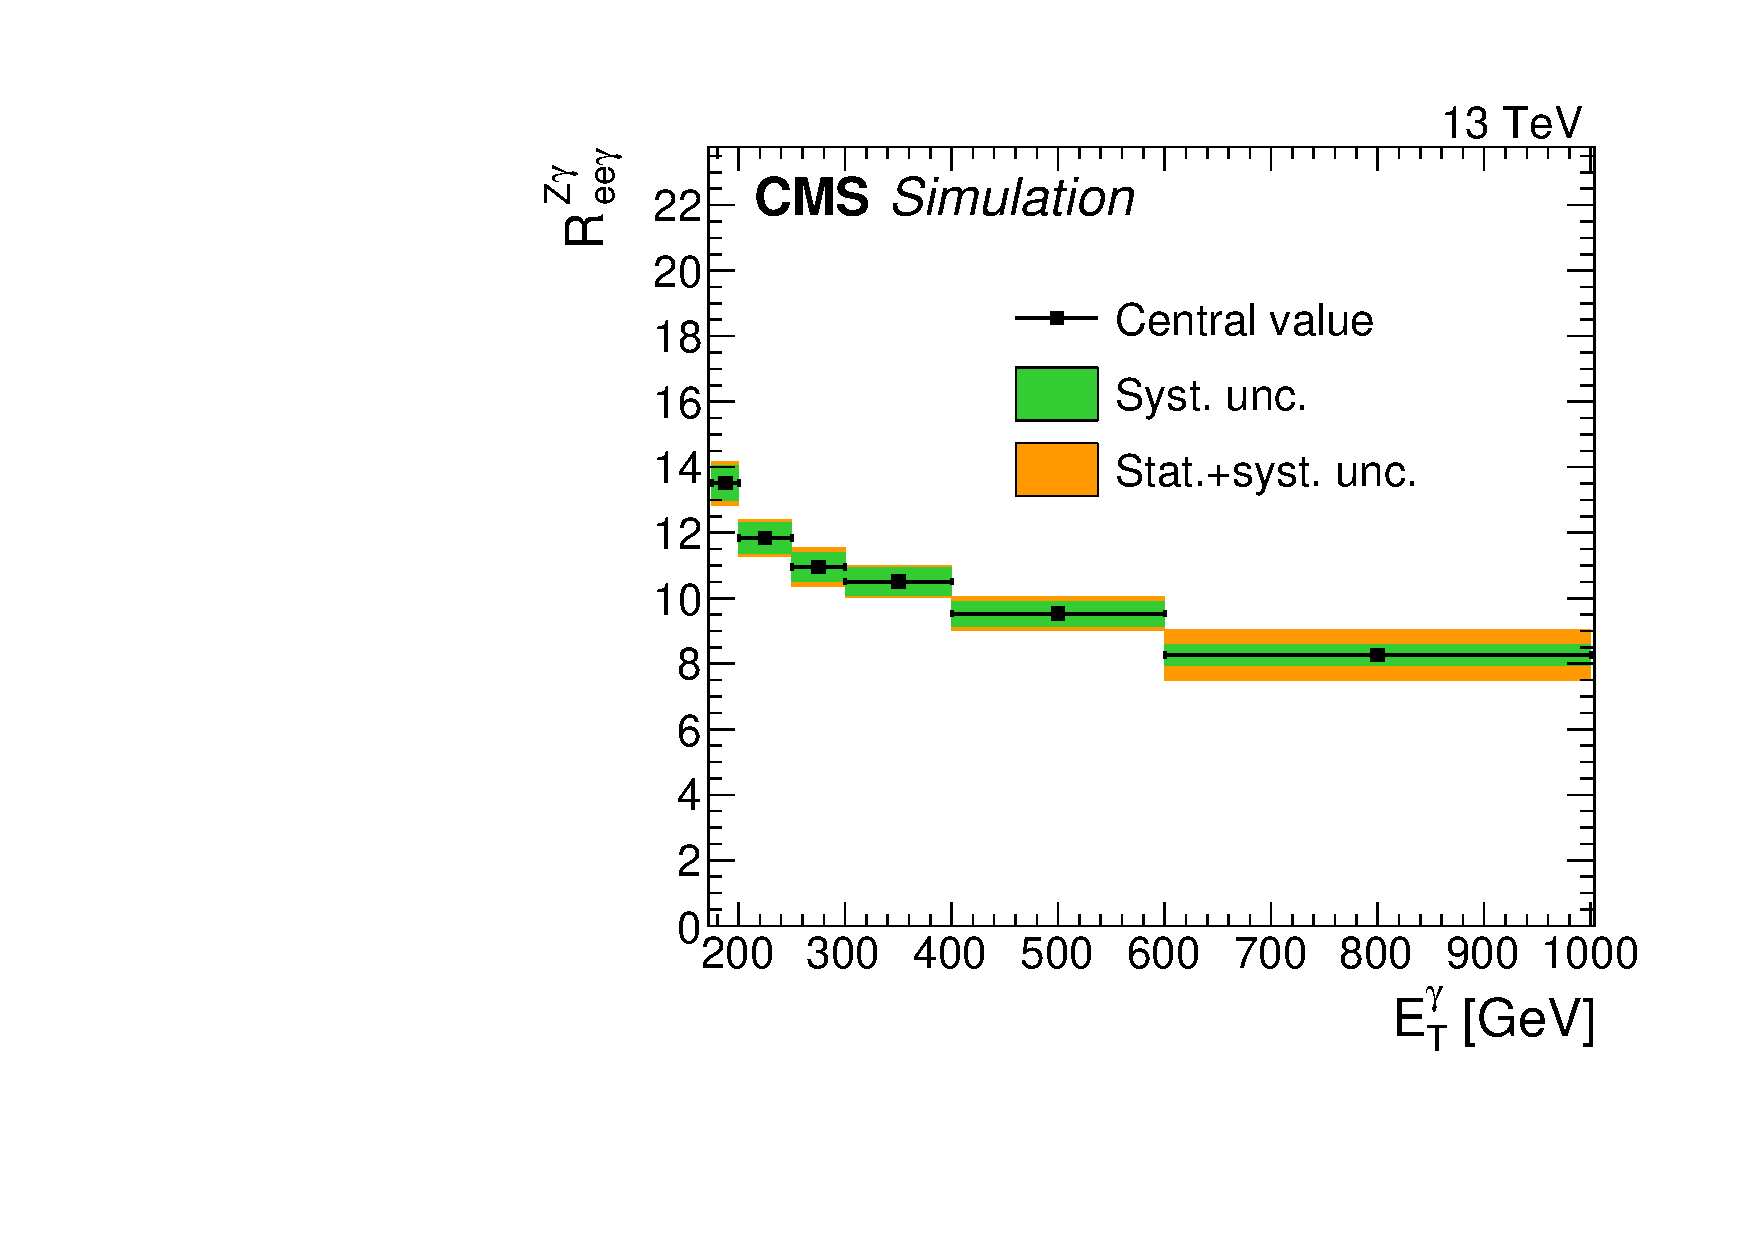
\includegraphics[width=0.49\textwidth]{Analysis/Figures/RZee.pdf}
    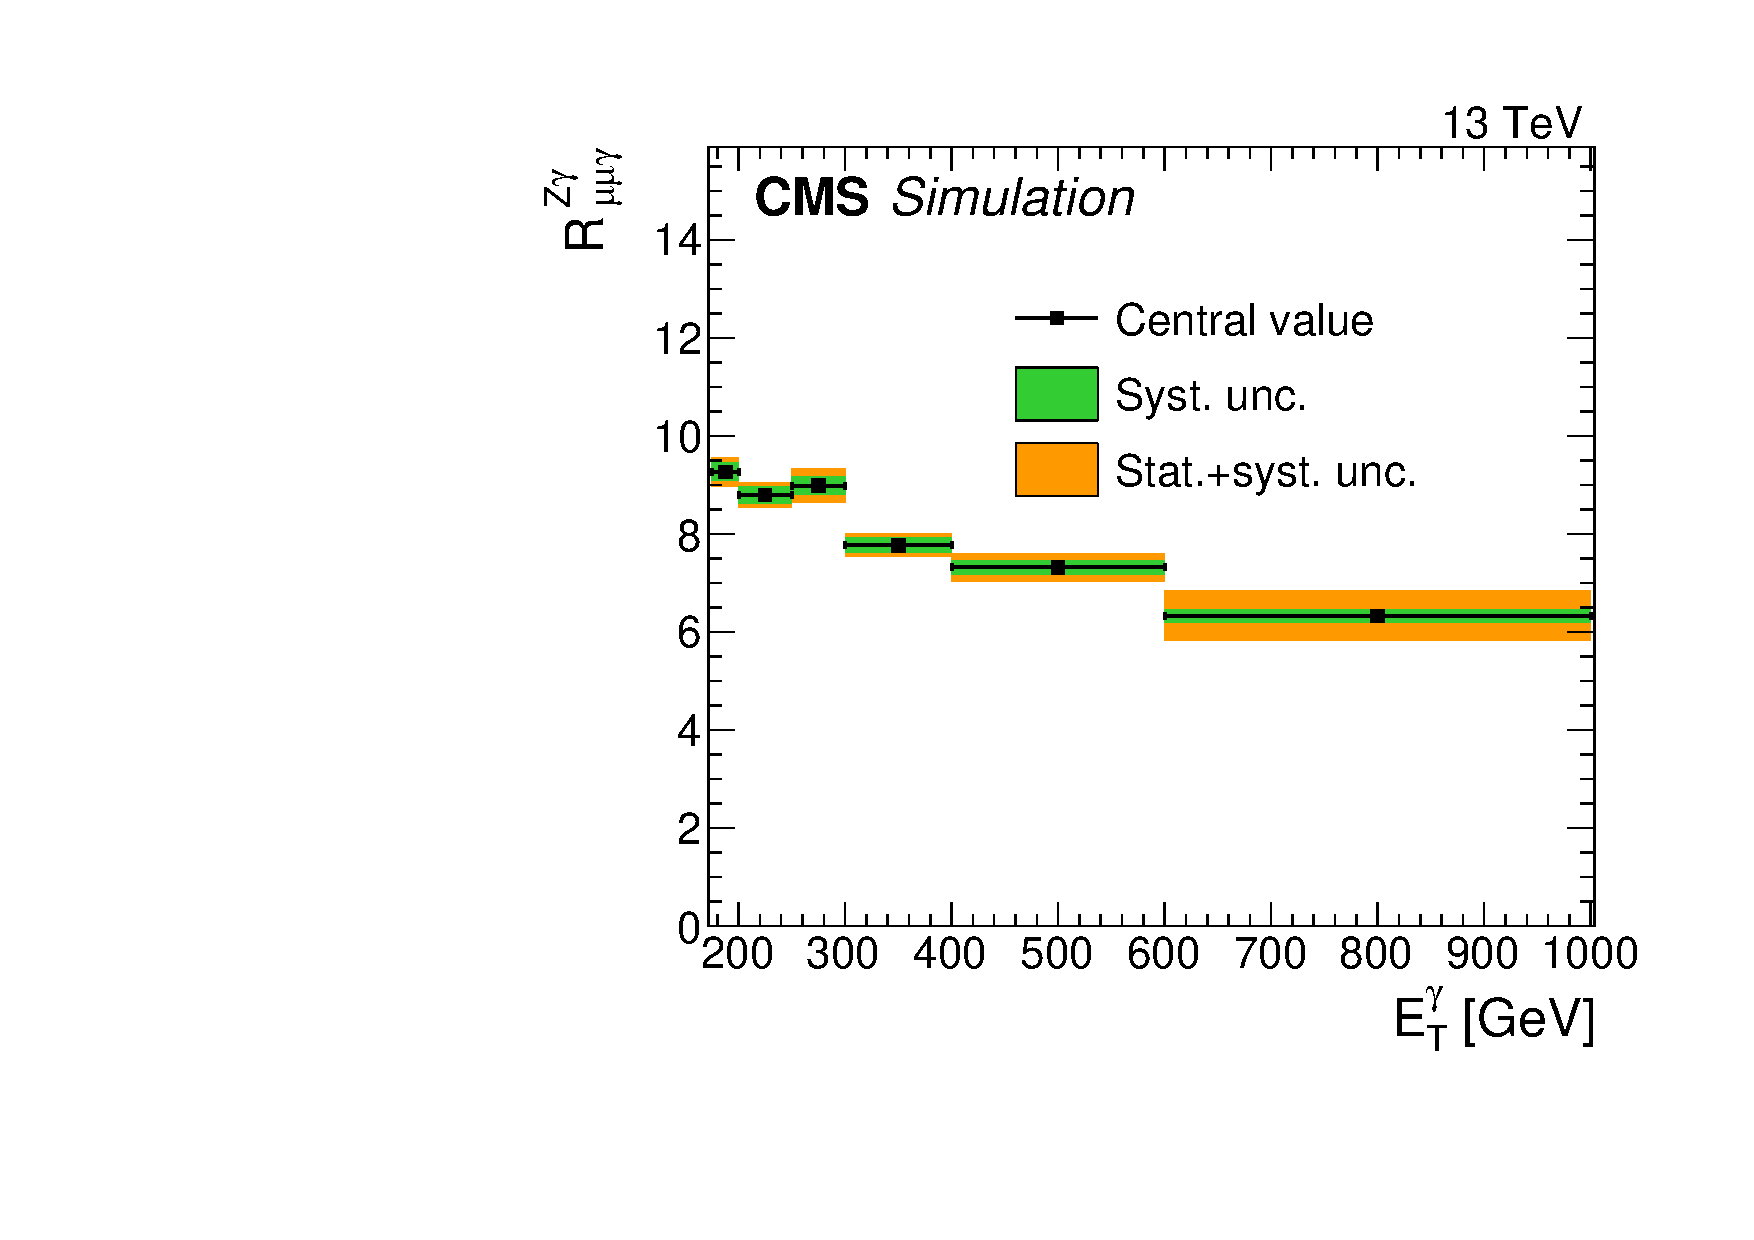
\includegraphics[width=0.49\textwidth]{Analysis/Figures/RZmm.pdf}
    \caption{
      Transfer factors \RZee\ (left) and \RZmm\ (right). 
      The uncertainty bands in green (inner) and orange (outer) show the systematic uncertainty, and the combination of systematic and statistical uncertainty arising from limited MC sample size, respectively. 
      The systematic uncertainties considered are the uncertainties in the data-to-simulation correction factors $\rho$ for the lepton identification efficiencies.
    }
    \label{fig:tf_z}
\end{figure}

Using the transfer factor \RZll, the total estimated event yield \Tll\ in each dilepton control region in the $i^\mathrm{th}$ bin of the \ETg\ distribution can be expressed as
\begin{equation}
  \Tll[,i] = \frac{\NZg[i]}{\RZll[,i]} + b_{\ell\ell\Pgg,i},
\end{equation}
where \NZg\ is the number of \zinvg\ events in the combined signal regions and $b_{\ell\ell\Pgg}$ is the predicted contribution from other background sources in the dilepton control region, namely \ttg, VV\Pgg, and misidentified hadrons. 
The subscript $i$ indicates that the quantities are evaluated in bin $i$ of the \ETg\ distribution.

\begin{figure}[htbp]
  \centering
    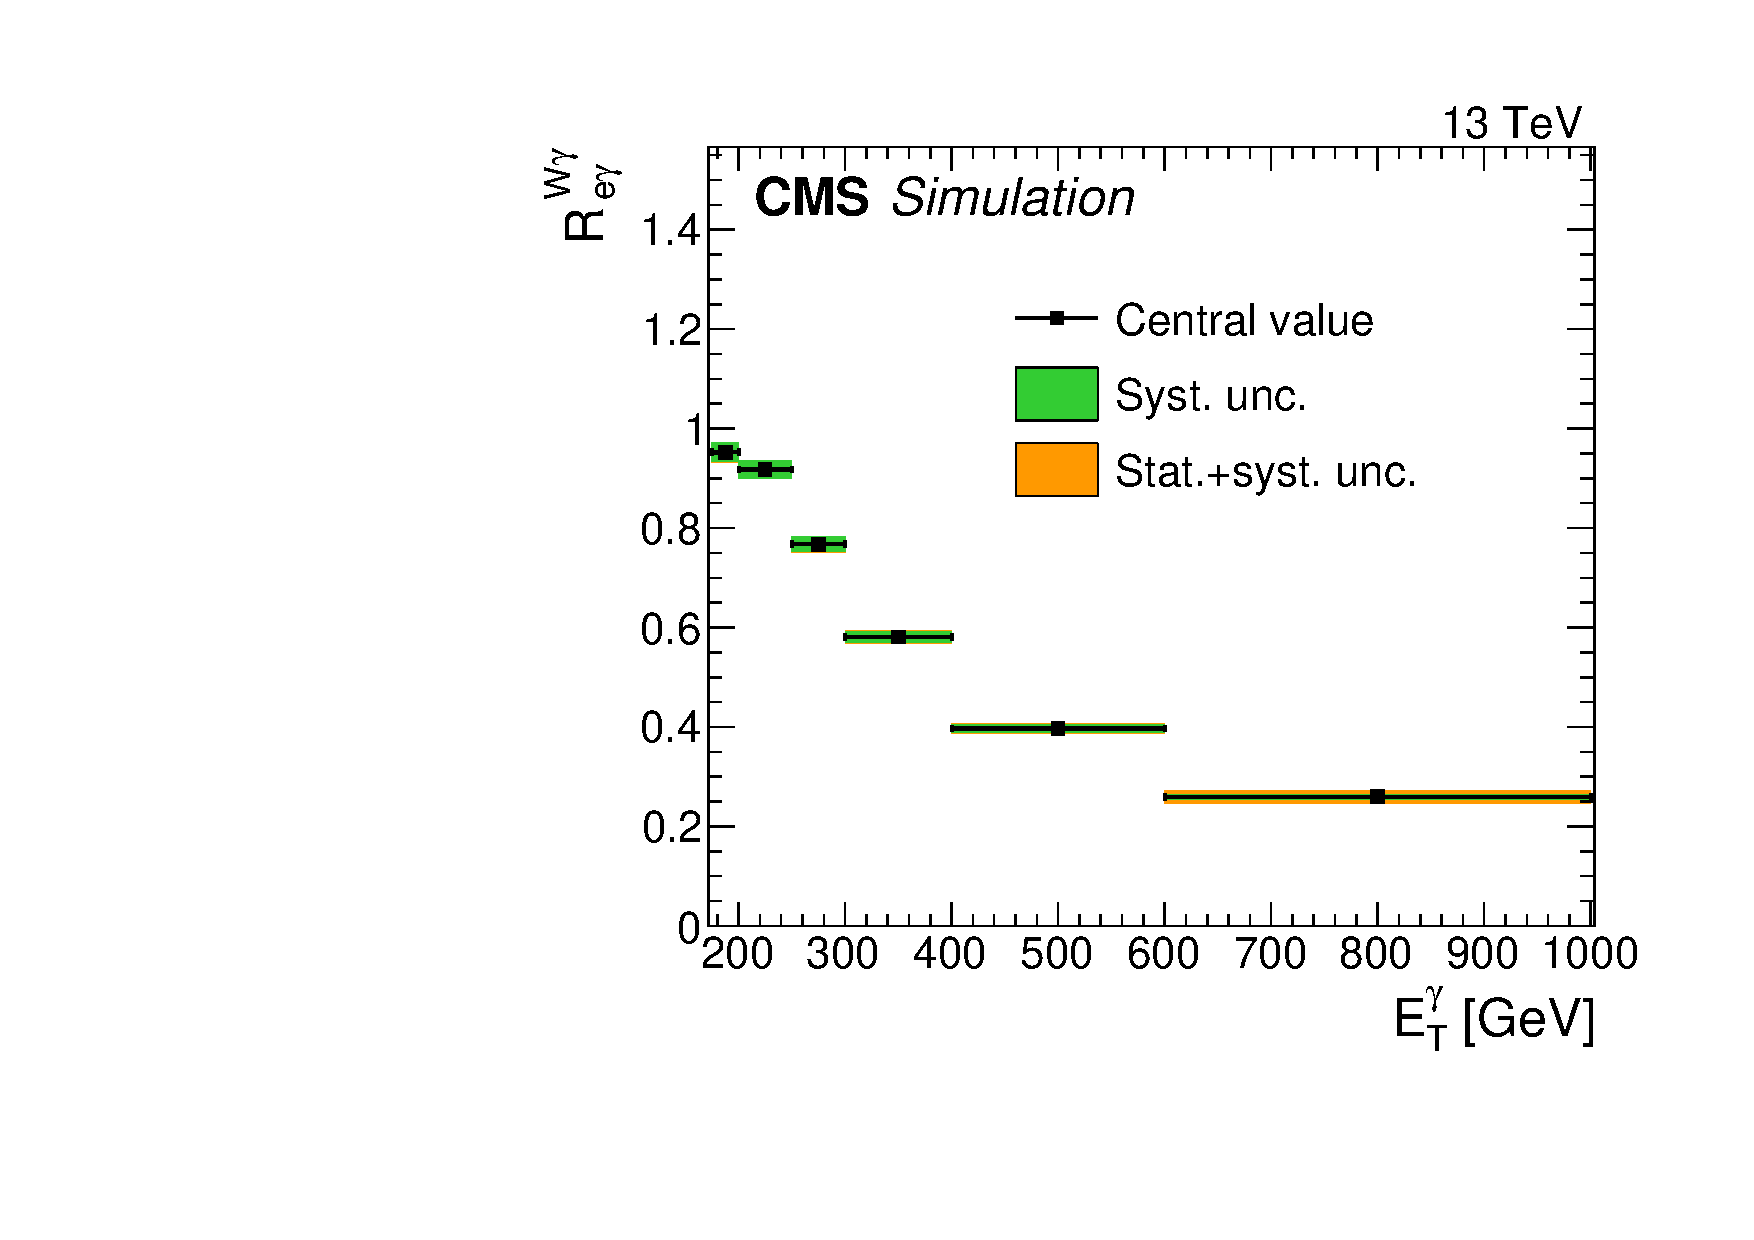
\includegraphics[width=0.49\textwidth]{Analysis/Figures/RWe.pdf}
    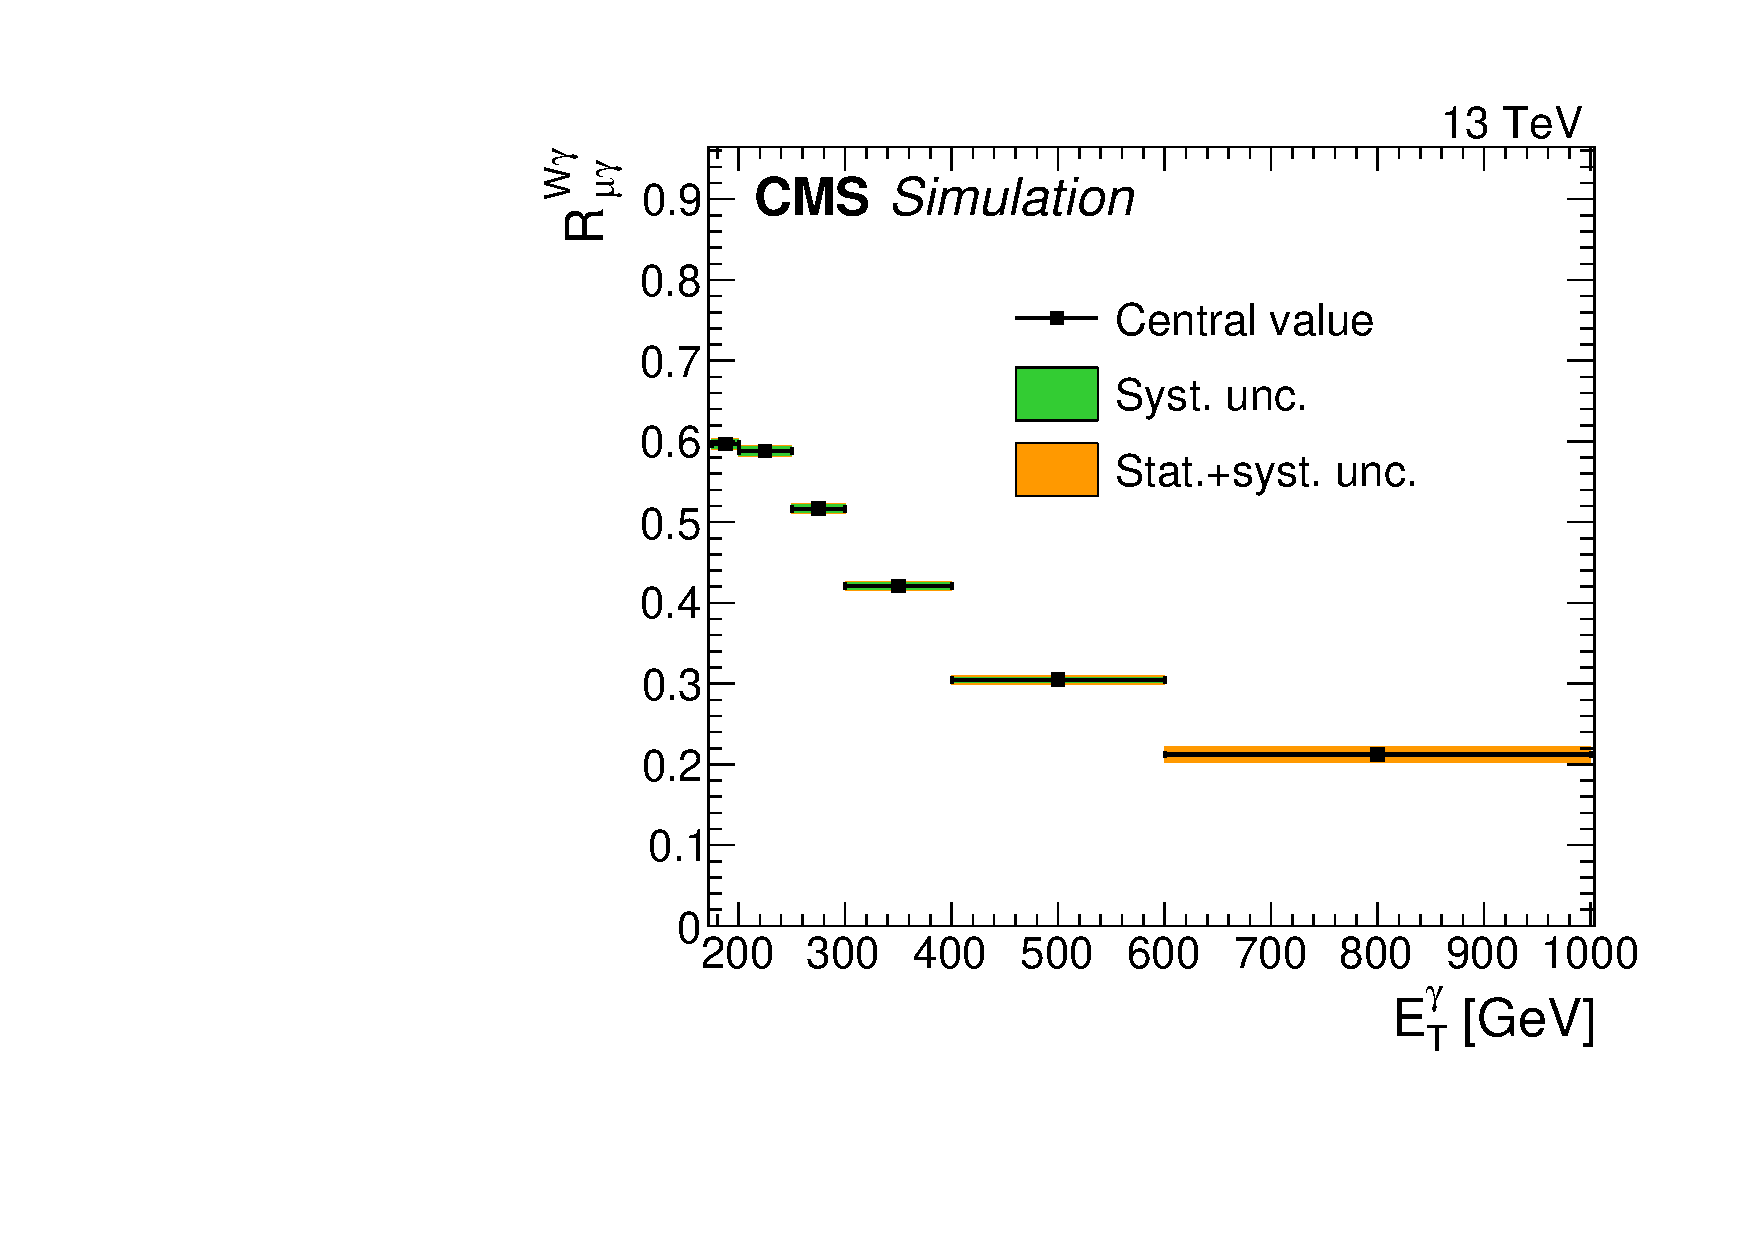
\includegraphics[width=0.49\textwidth]{Analysis/Figures/RWm.pdf}
    \caption{
      Transfer factors \RWe\ (left) and \RWm\ (right). 
      The uncertainty bands in green (inner) and orange (outer) show the systematic uncertainty, and the combination of systematic and statistical uncertainty arising from limited MC sample size, respectively. 
      The systematic uncertainties considered are the uncertainties in the data-to-simulation correction factors $\rho$ for the lepton identification efficiencies.
    }
    \label{fig:tf_w}
\end{figure}

\begin{figure}[htbp]
  \centering
    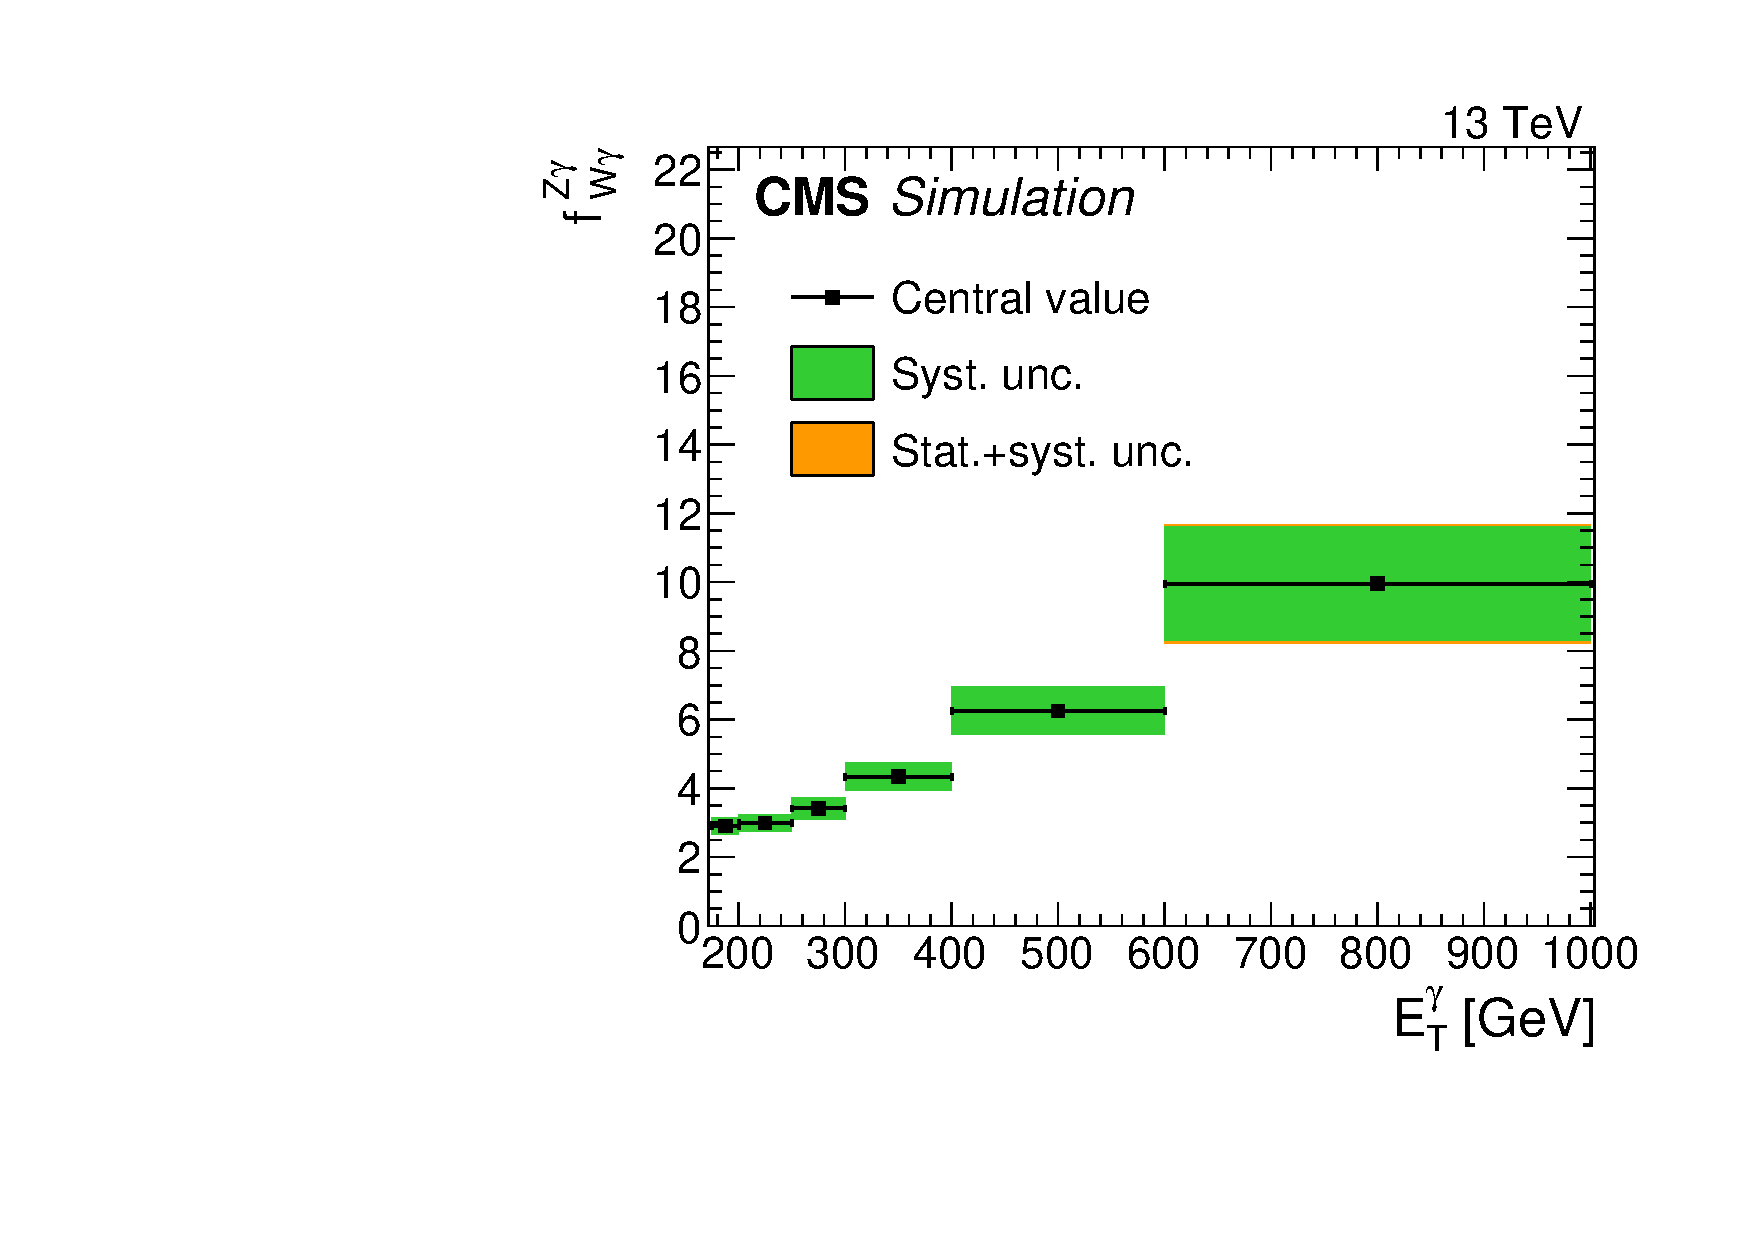
\includegraphics[width=0.49\textwidth]{Analysis/Figures/fZW.pdf}
    \caption{
      Transfer factor \fZW. 
      The uncertainty bands in green (inner) and orange (outer) show the systematic uncertainty, and the combination of systematic and statistical uncertainty arising from limited MC sample size, respectively. 
      The systematic uncertainties considered are the uncertainties from higher-order theoretical corrections.
    }
    \label{fig:tf_wz}
\end{figure}

Using \RWl\ and \fZW, the total estimated event yield \Tl\ in each single-lepton control region in the $i^\mathrm{th}$ bin of the \ETg\ distribution can be expressed as
\begin{equation}
  \Tl[,i] = \frac{\NZg[i]}{\RWl[,i]\fZW[,i]} + b_{\ell\Pgg,i},
\end{equation}
where $b_{\ell\Pgg}$ is the predicted contribution from other background sources in the single-lepton regions, namely misidentified electrons and hadrons and other minor SM processes.

\subsection{Higher-order corrections to \vg\ differential cross sections}
\label{sec:theory_uncertainties}

\begin{figure}[htbp]
  \centering
  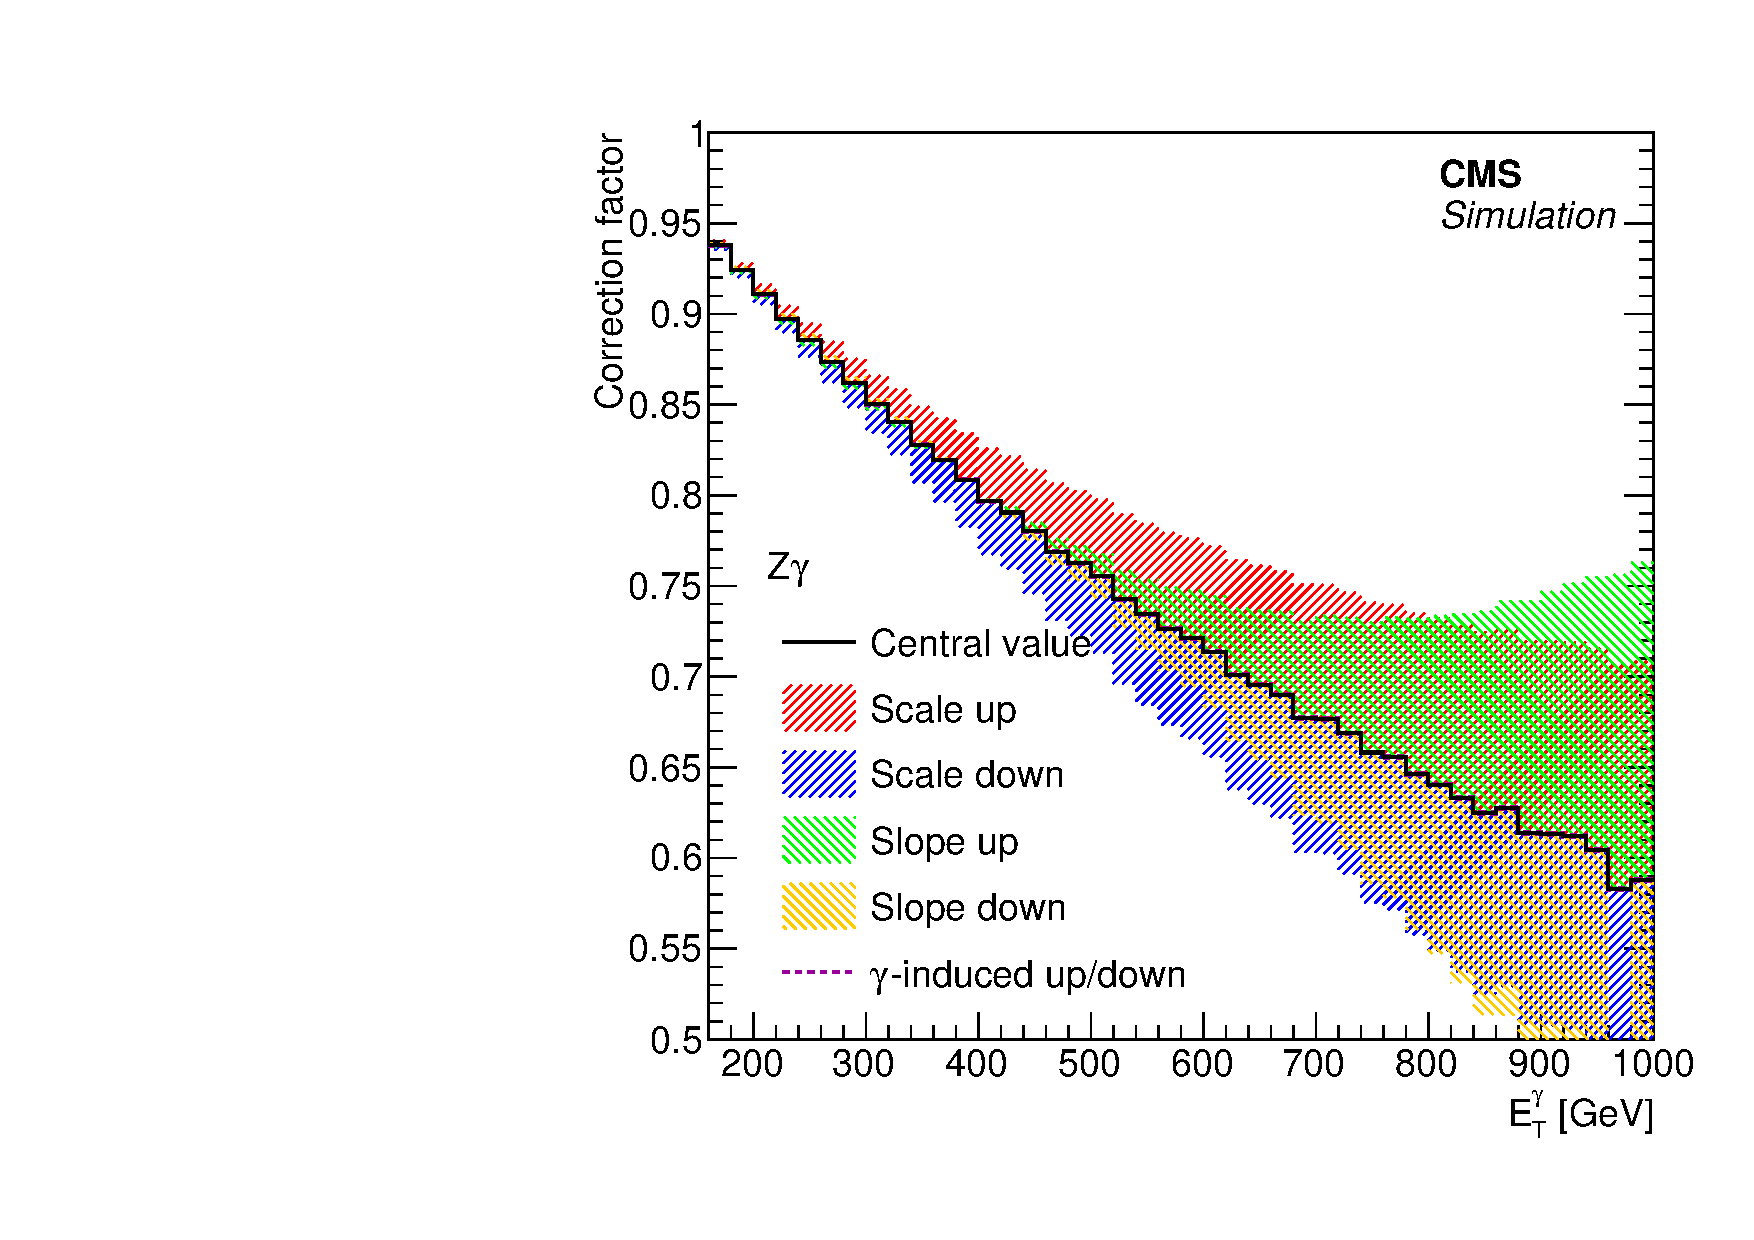
\includegraphics[width=0.48\linewidth]{Analysis/Figures/ewkcorr_zg.pdf} \\
  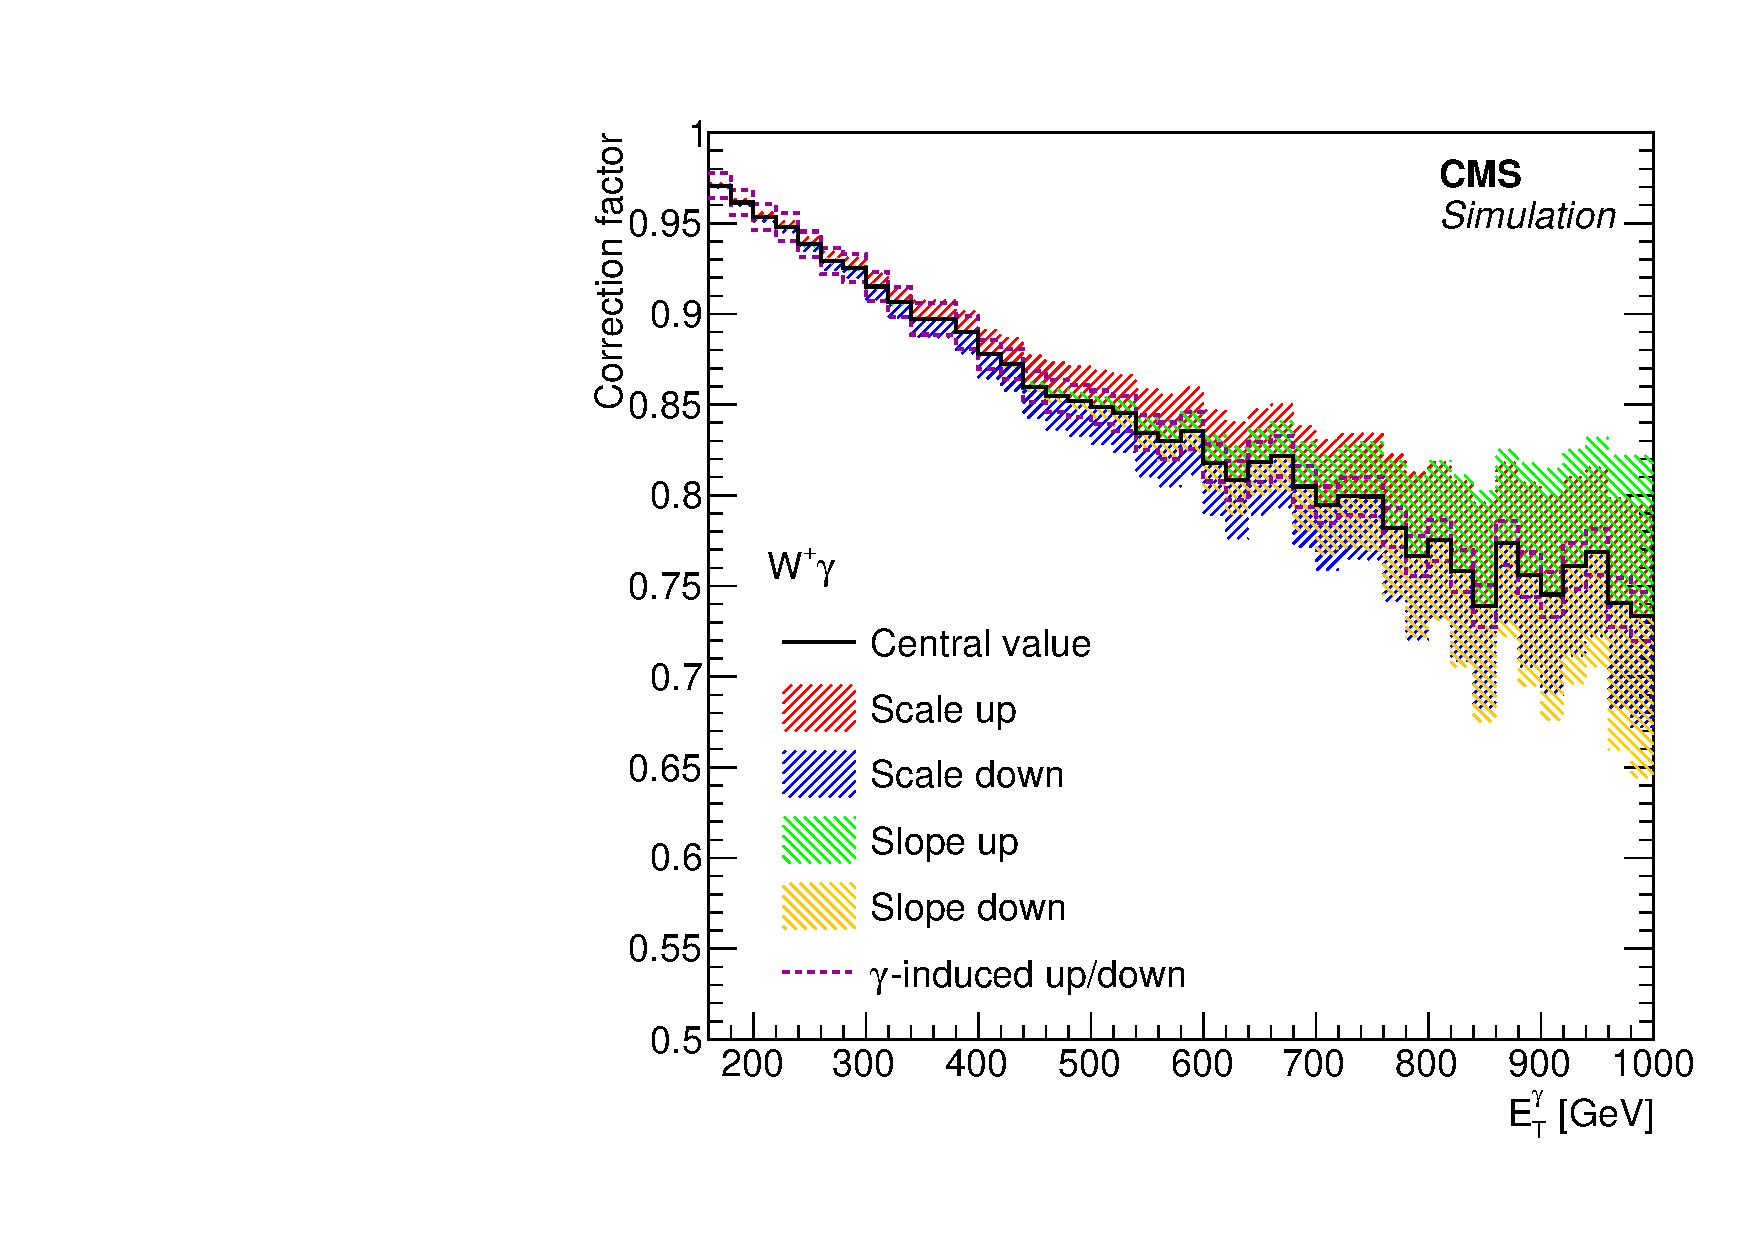
\includegraphics[width=0.48\linewidth]{Analysis/Figures/ewkcorr_wgplus.pdf}
  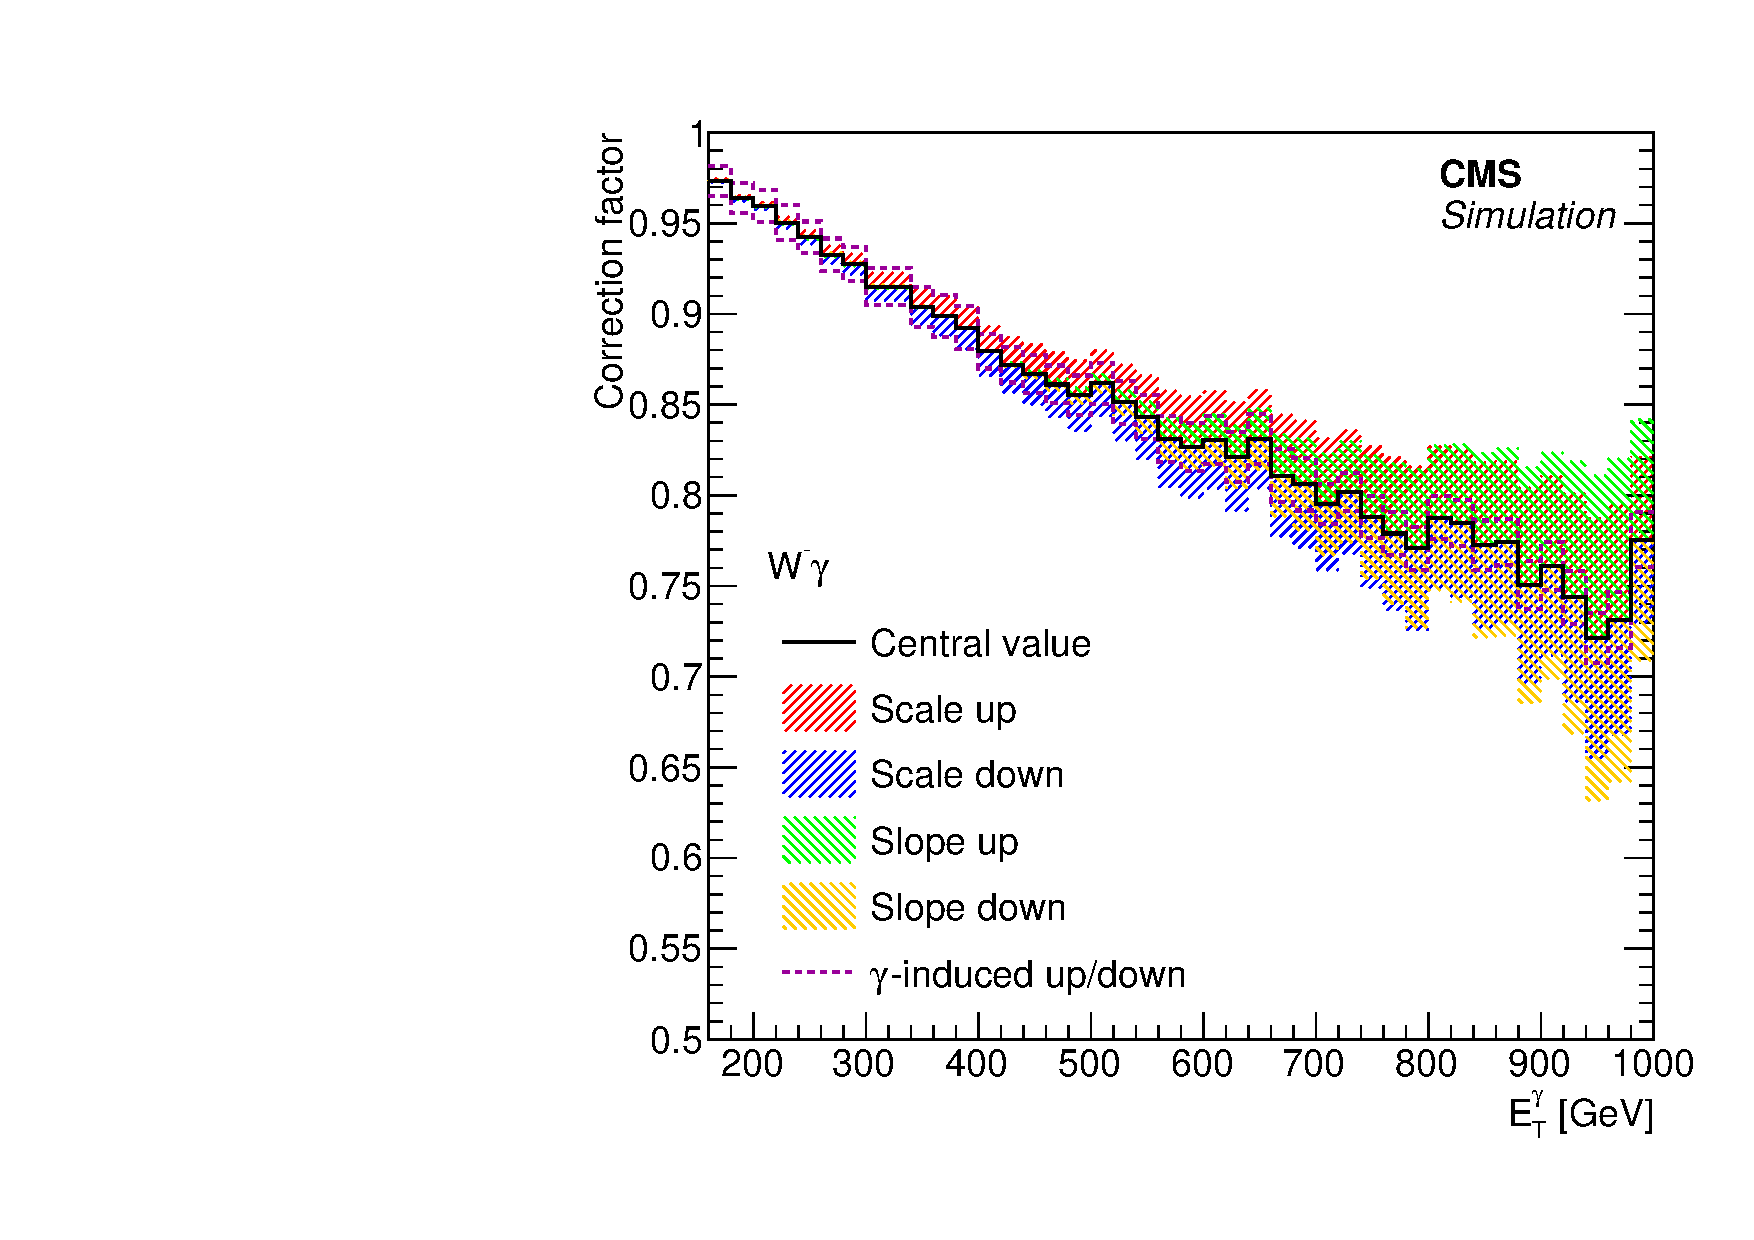
\includegraphics[width=0.48\linewidth]{Analysis/Figures/ewkcorr_wgminus.pdf}
  \caption{
    Electroweak NLO cross section corrections as a function of photon \PT for \zinvg\ (top), $\PW^{+}+\Pgg$ (bottom left), and $\PW^{-}+\Pgg$ (bottom right) processes, overlaid with uncertainty bands. 
    See text for descriptions of the individual components of the uncertainty.
    The uncertainty due to \Pgg-induced production is negligible in \zinvg\ production.
  }
  \label{fig:ewk_correction}
\end{figure}

We apply the correction factors shown in Fig.~\ref{fig:ewk_correction}, which are combinations of Sudakov suppression factors and photon-induced enhancements, and are provided by the authors of Ref.~\cite{Denner:2015fca} in addition to the NNLO QCD correction.

\begin{figure}[htbp]
  \centering
    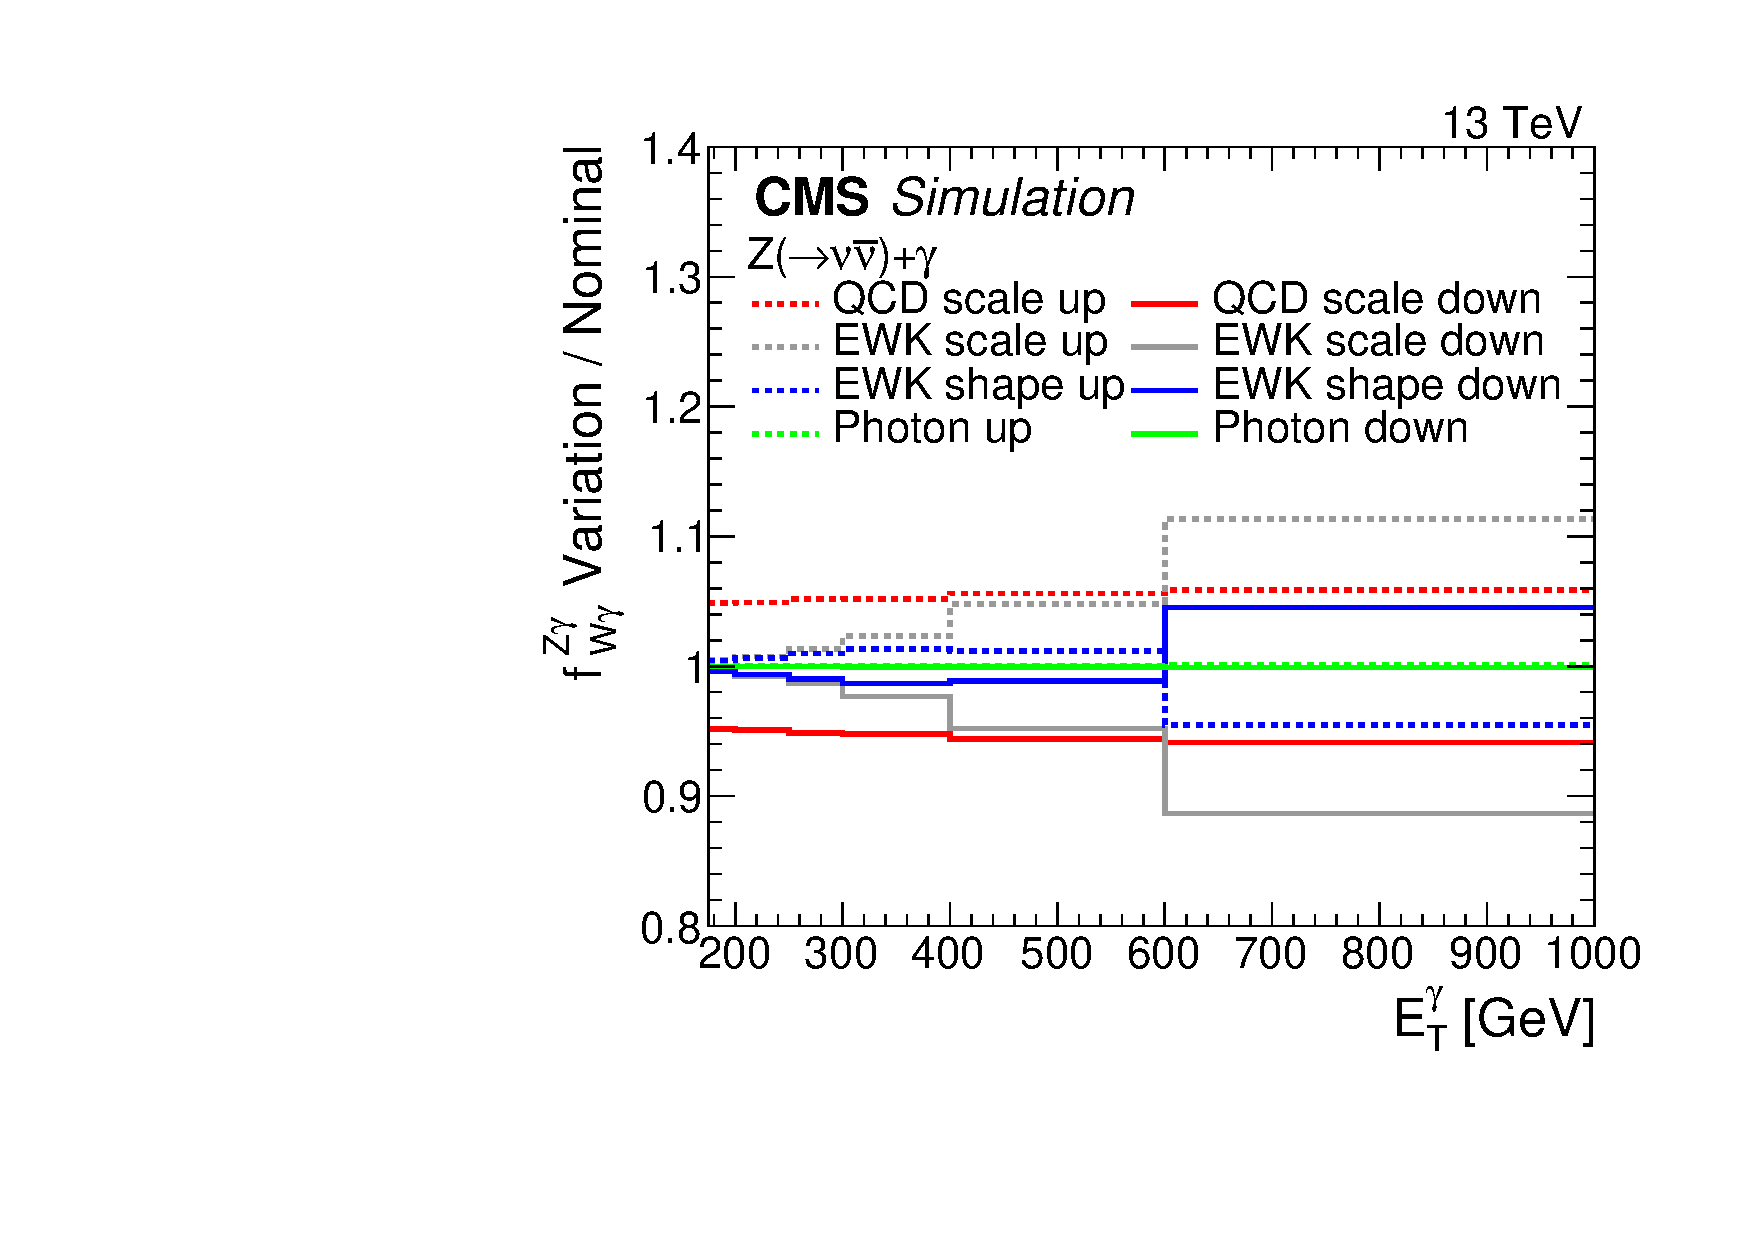
\includegraphics[width=0.45\textwidth]{Analysis/Figures/tf_syst_zg.pdf}
    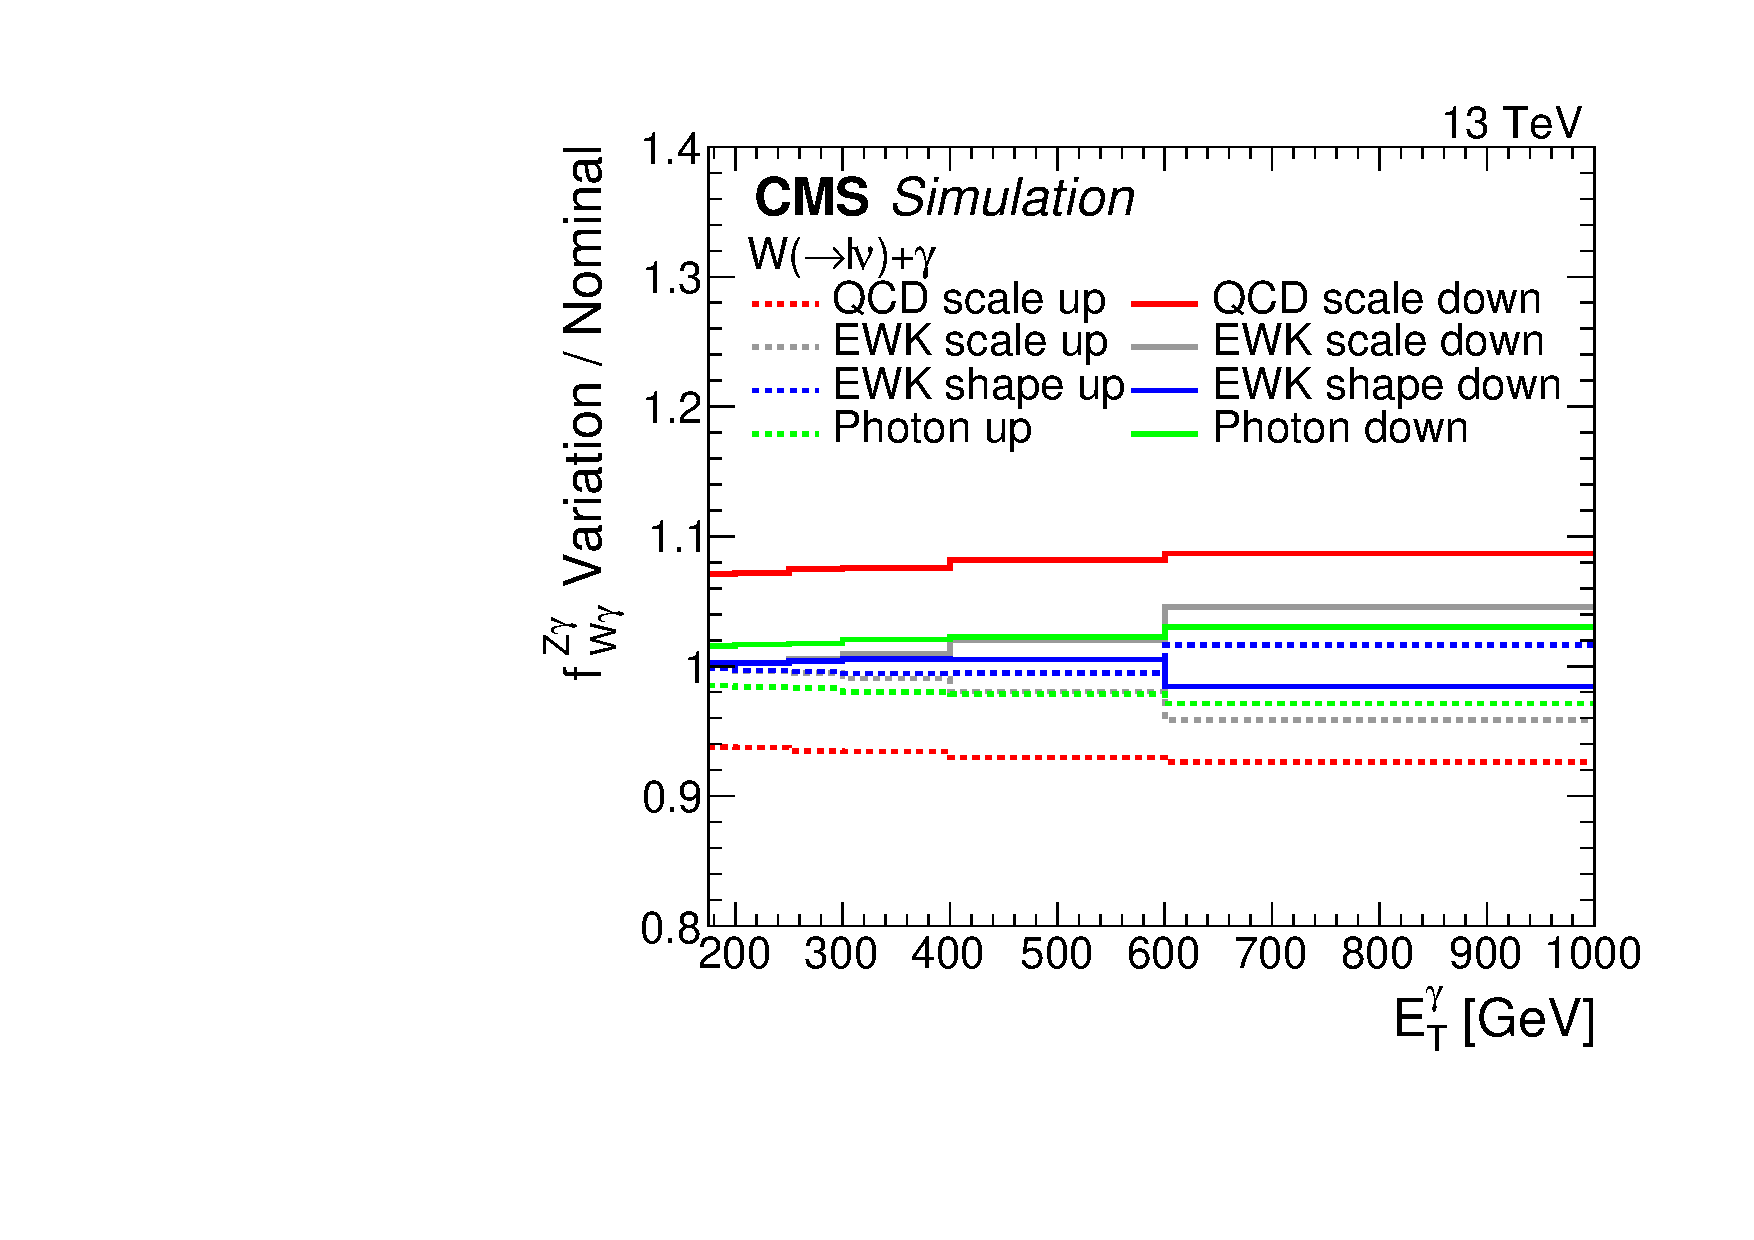
\includegraphics[width=0.45\textwidth]{Analysis/Figures/tf_syst_wg.pdf}
    \caption{
      Systematic uncertainty in the transfer factors for \zinvg\ (left) and \wlng\ (right). The last bin includes all events with $\ETg > 1000\GeV$.
    }
    \label{fig:tf_syst}
\end{figure}

Figure~\ref{fig:tf_syst} shows the effect of systematic uncertainty in the ratio between the \zinvg\ and \wlng\ processes with respect to nominal value for ${\PZ\Pgg}$ and ${\PW\Pgg}$ respectively.

\section{Misidentified electrons}
\label{sec:efake}

\section{Misidentified hadrons}
\label{sec:hfake}

\section{Spikes}
\label{sec:spikes}

\section{Beam halo}
\label{sec:beam_halo}

The splitting of the signal region can be thought of as a two-bin fit. 
Collision processes occupy the relative fractions of phase space in the horizontal ($H$) and vertical ($V$) signal regions, $C_{H} = 1/\pi$ and $C_{V} = (\pi-1)/\pi$, respectively. 
The corresponding fractions for beam halo events are determined by selecting a halo-enriched sample where the halo identification is inverted. 
Thus, a fit of the two signal regions provides an estimate of the overall normalization of the beam halo background, denoted $h$. 
The \ETg\ dependence of the halo background is encoded in \nhalo[,i], the unit-normalized beam halo prediction in the $i^\mathrm{th}$ bin of the signal region $K \in \{H,V\}$.
Using the notation introduced in Section~\ref{sec:irreducible}, the total estimated background \TK\ in the two signal regions are
\begin{equation}
\begin{aligned}
  \TK[,i] & = C_{K} (\NZg[i] + \NWg[i]) + h \nhalo[,i] + C_{K} b_{K,i} \\
          & = C_{K} (1 + {\fZW[i]}^{-1}) \NZg[i] + h \nhalo[,i] + C_{K} b_{K,i},
\end{aligned}
\end{equation}
where $b_{K,i}$ is the total contribution to bin $i$ of region $K$ from electron and hadron misidentification, ECAL spikes, and other minor SM background processes.

\section{Other minor SM background processes}
\label{sec:minorsm}
The SM \ttg, VV\Pgg, \zllg, $\PW\to\ell\PGn$, and \gj\ processes are minor ($\sim$10\%) background processes in the signal region. 
Although \zllg\ and \gj\ do not involve high-\PT invisible particles, the former can exhibit large \met when the leptons fail to be reconstructed, and the latter when jet energy is severely mismeasured. 
The estimates for all five processes are taken from \MGvATNLO simulations at LO in QCD and can be found in Tables~\ref{tab:yield_mask_horizontal} and~\ref{tab:yield_mask_vertical}.

\section{Statistical Interpretation}
\label{sec:interpretation}

Free parameters of the fit are the yield of \zinvg\ background in each bin of the signal regions (\NZg[i]) and the overall normalization of the beam halo background ($h$). 
Bin-by-bin yields of \wlng\ and \zllg\ samples in all regions are related to the yield of \zinvg\ through the MC prediction through the transfer factors defined in Section~\ref{sec:irreducible}. 
The transfer factors are allowed to shift within the aforementioned theoretical and experimental uncertainties.

The background-only likelihood that is maximized in the fit is
\begin{equation}
\begin{aligned}
  \mathcal{L} & = \prod_{i} \left\{ \mathcal{L_{\text{signal}}} \times \mathcal{L_{\text{single-lepton}}} \times \mathcal{L_{\text{dilepton}}} \right\} \times \mathcal{L_{\text{nuisances}}} \\
  & = \prod_{i} \left\{
    \prod_{K=H,V} \mathcal{P}\left( d_{K, i} \left| \TK[,i] (\vec{\theta} \right.) \right) \times \prod_{\ell=\Pe,\Pgm} \mathcal{P}\left( d_{\ell\Pgg, i} \left| \Tl[,i] (\vec{\theta}) \right. \right)
    \times \prod_{\ell=\Pe,\Pgm} \mathcal{P}\left( d_{\ell\ell\Pgg, i} \left| \Tll[,i] (\vec{\theta}) \right. \right)
    \right\}  \times \prod_{j} \mathcal{N}(\theta_j) \\
  & = \prod_{i} \left\{
  \begin{gathered}
    \prod\limits_{K=H,V} \mathcal{P}\biggl( d_{K, i} \biggl| \left(1 + {\fZW[,i]}^{-1}(\vec{\theta})\right) C_{K} \NZg[i] + h \nhalo[,i](\vec{\theta}) + C_{K} b_{K, i}(\vec{\theta}) \biggr. \biggr) \\
    \times \prod\limits_{\ell=\Pe,\Pgm} \mathcal{P}\biggl( d_{\ell\Pgg, i} \biggl| \frac{\NZg[i]}{\RWl[,i](\vec{\theta}) \fZW[,i] (\vec{\theta})} + b_{\ell\Pgg, i}(\vec{\theta}) \biggr. \biggr) \\
    \times \prod\limits_{\ell=\Pe,\Pgm} \mathcal{P}\biggl( d_{\ell\ell\Pgg, i} \biggl| \frac{\NZg[i]}{\RZll[,i](\vec{\theta})} + b_{\ell\ell\Pgg, i}(\vec{\theta}) \biggr. \biggr)
  \end{gathered} \right\}
  \times \prod_{j} \mathcal{N}(\theta_j),
\end{aligned}
\end{equation}
following the notation introduced in Section~\ref{sec:irreducible}, and where $\mathcal{P}
(n\vert\lambda)$ is the Poisson probability of $n$ for mean $\lambda$, $\mathcal{N}$ denotes the unit normal distribution, and $d_{X,i}$ is the observed number of events in bin i of region X.
Systematic uncertainties are treated as nuisance parameters in the fit and are represented by
$\vec{\theta}$.
Each quantity $Q_{j}$ with a nominal value $\overline{Q}_{j}$ and a standard deviation of the systematic uncertainty $\sigma_{j}$ appears in the likelihood function as $\overline{Q}_{j}\exp(\sigma_{j}\theta_{j})$.

\section{Results}
\label{sec:results}

\subsection{Pre-fit and post-fit distributions}
\label{subsec:distributions}

\begin{figure}[htbp]
  \centering
    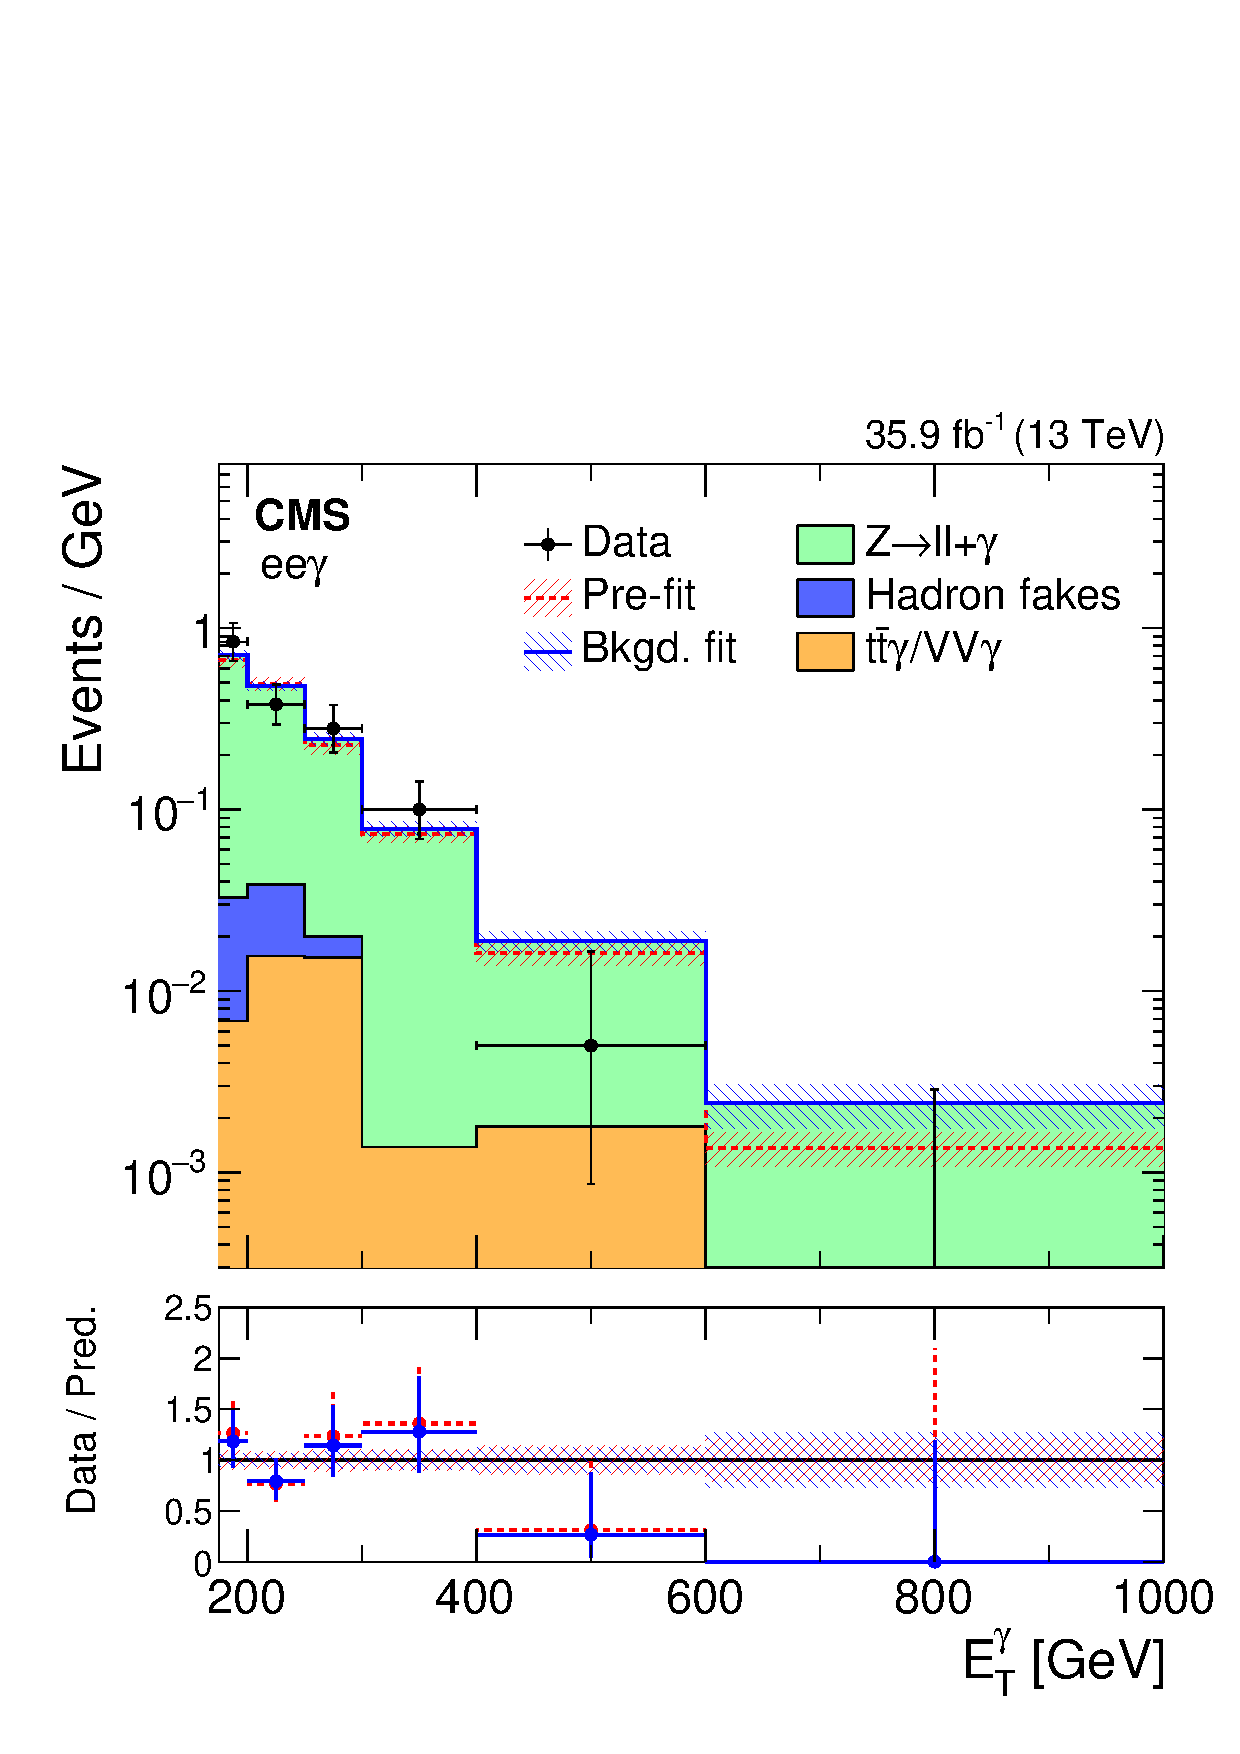
\includegraphics[width=0.45\textwidth]{Analysis/Figures/bonly_diel.pdf}
    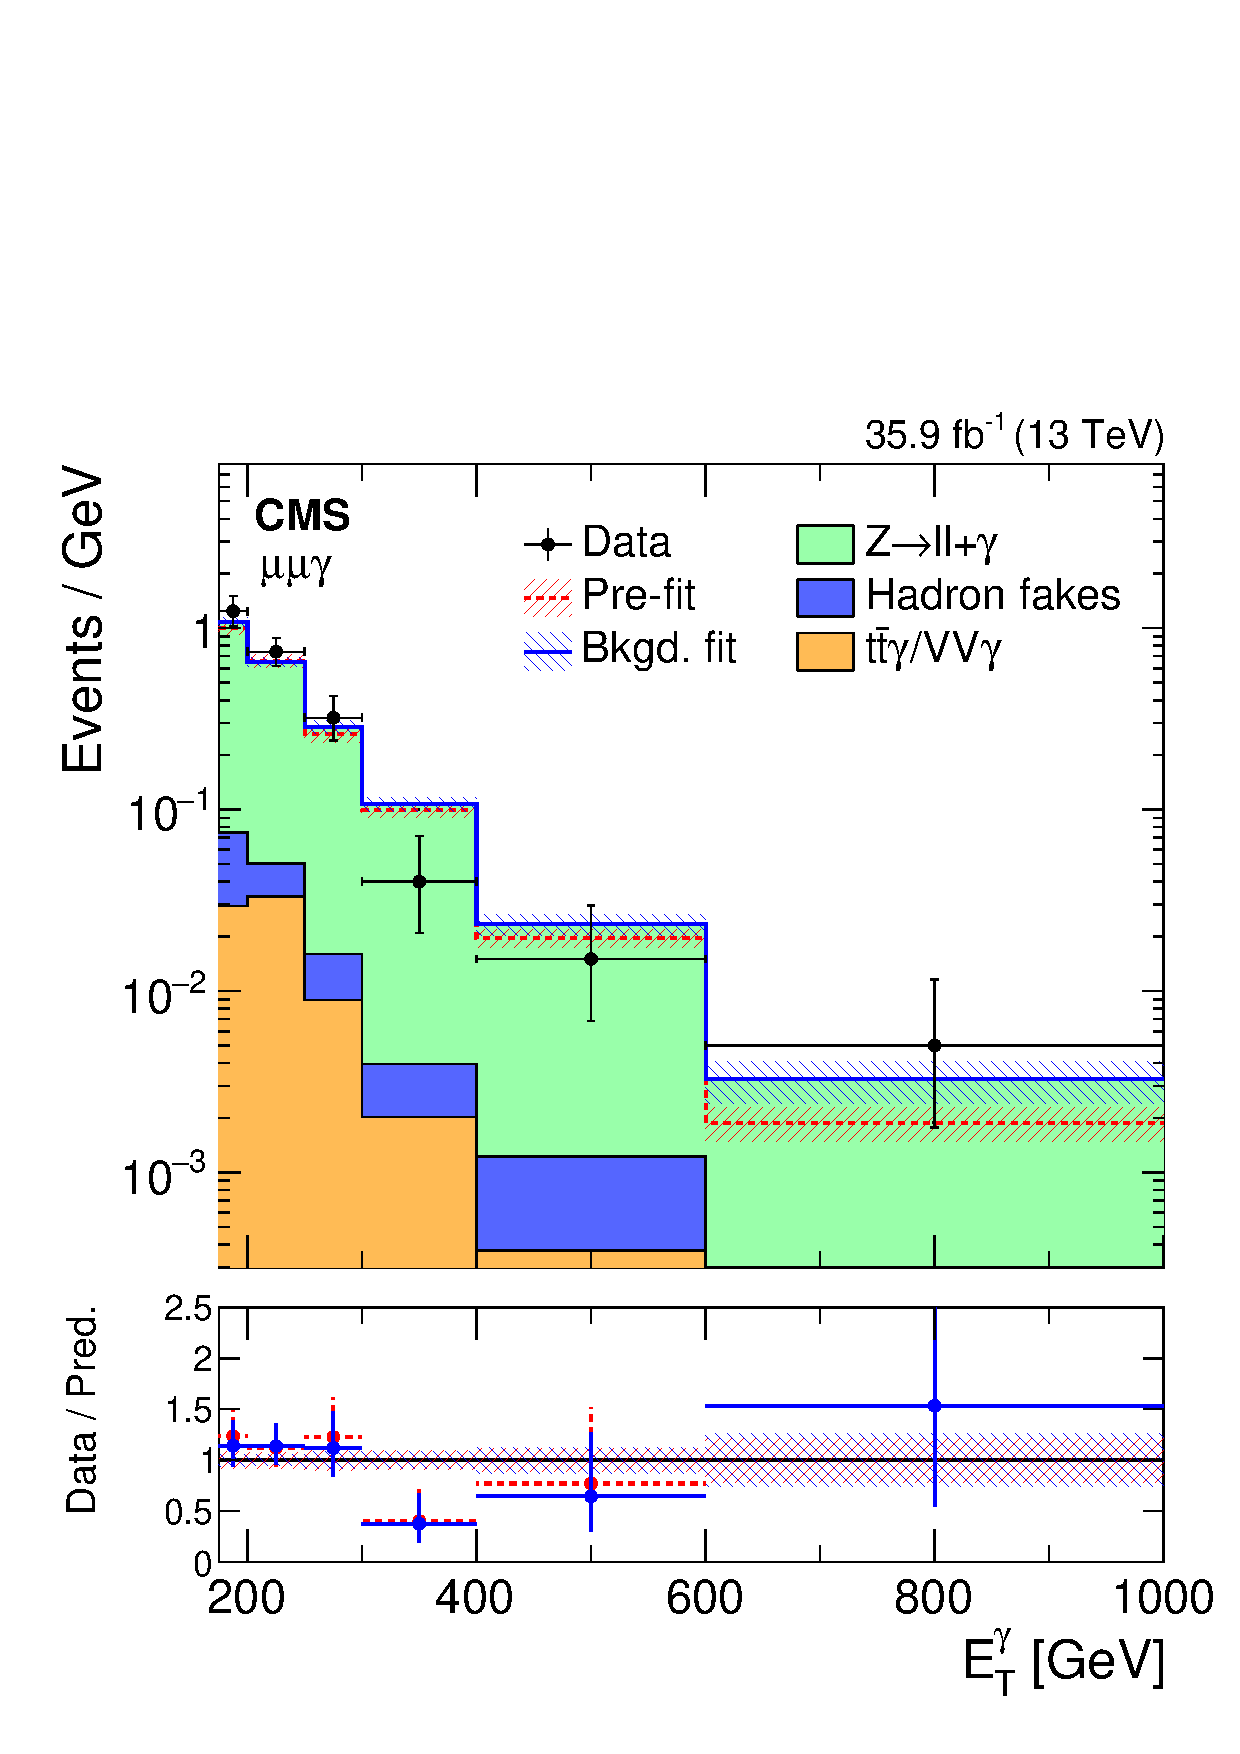
\includegraphics[width=0.45\textwidth]{Analysis/Figures/bonly_dimu.pdf}
    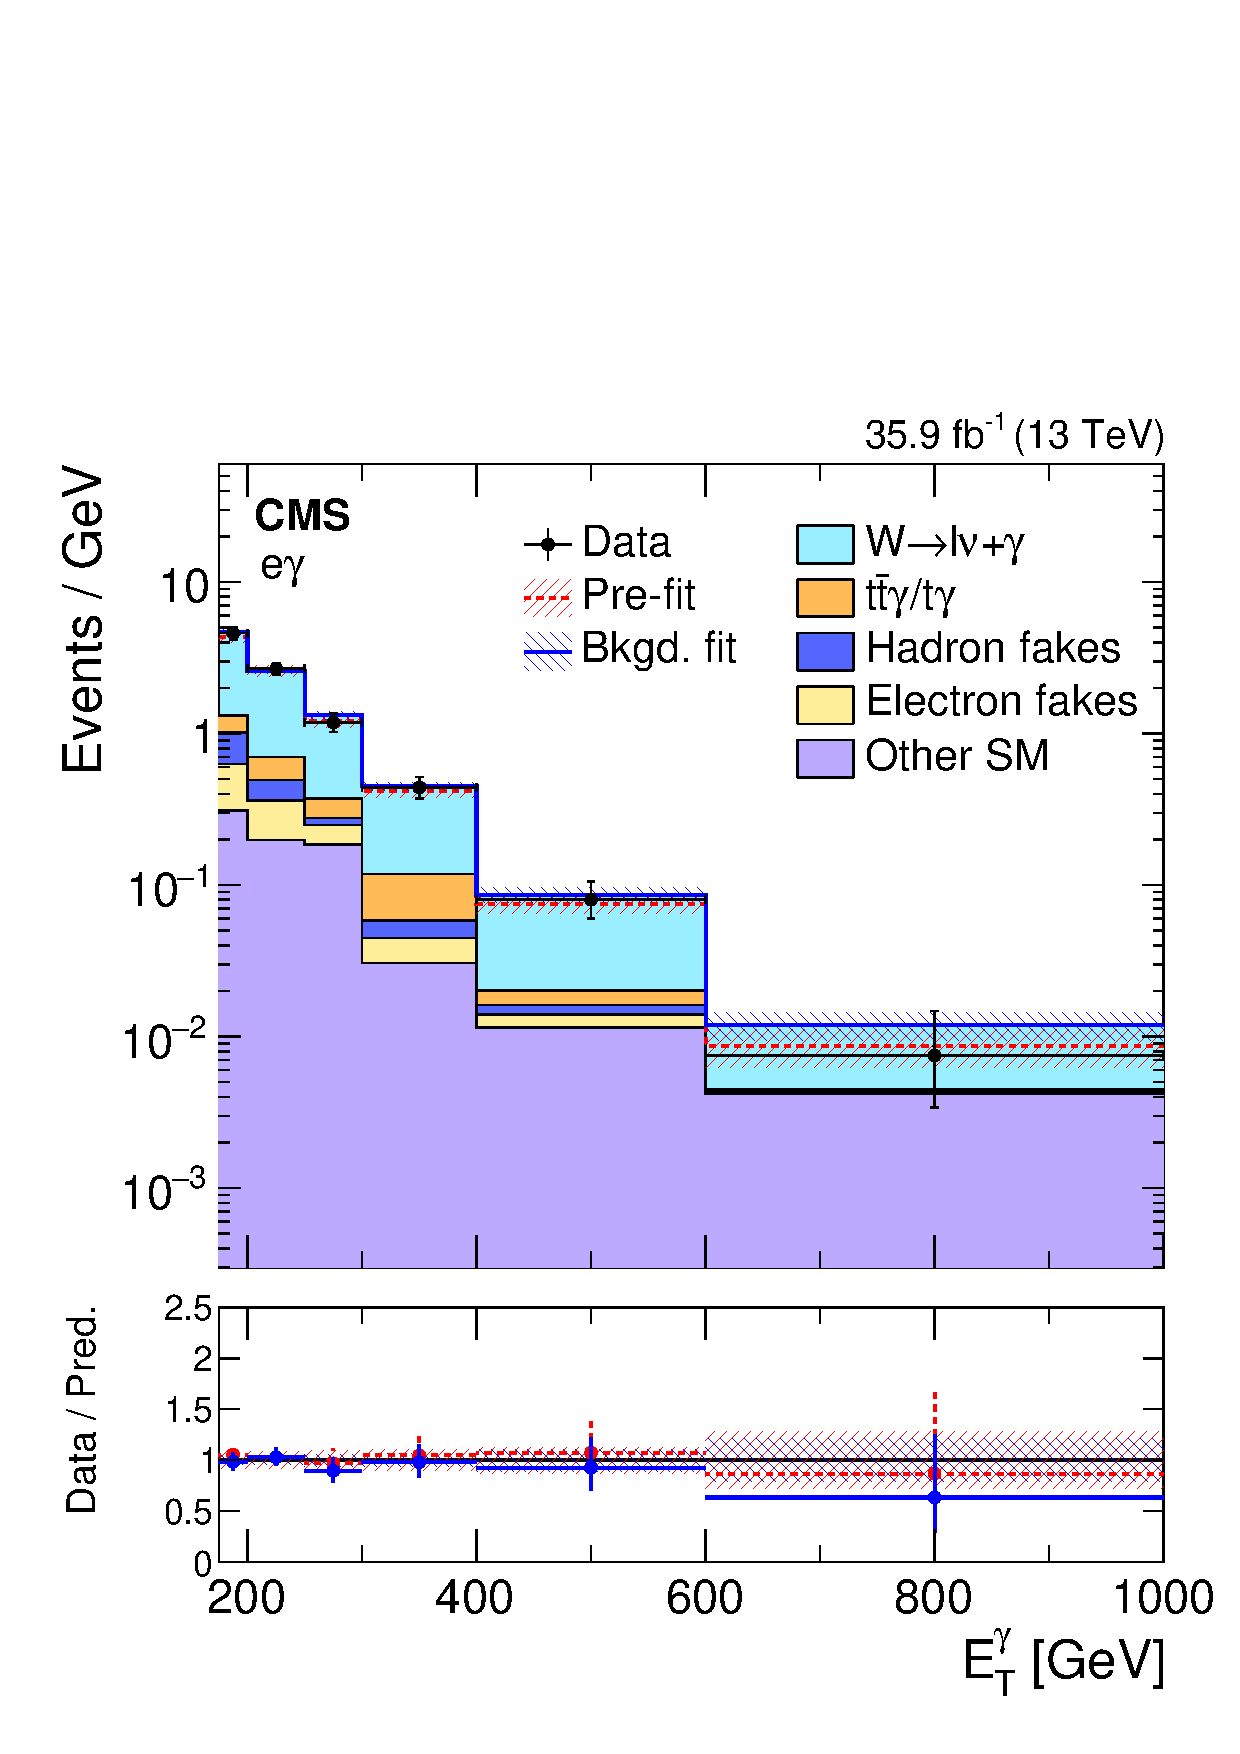
\includegraphics[width=0.45\textwidth]{Analysis/Figures/bonly_monoel.pdf}
    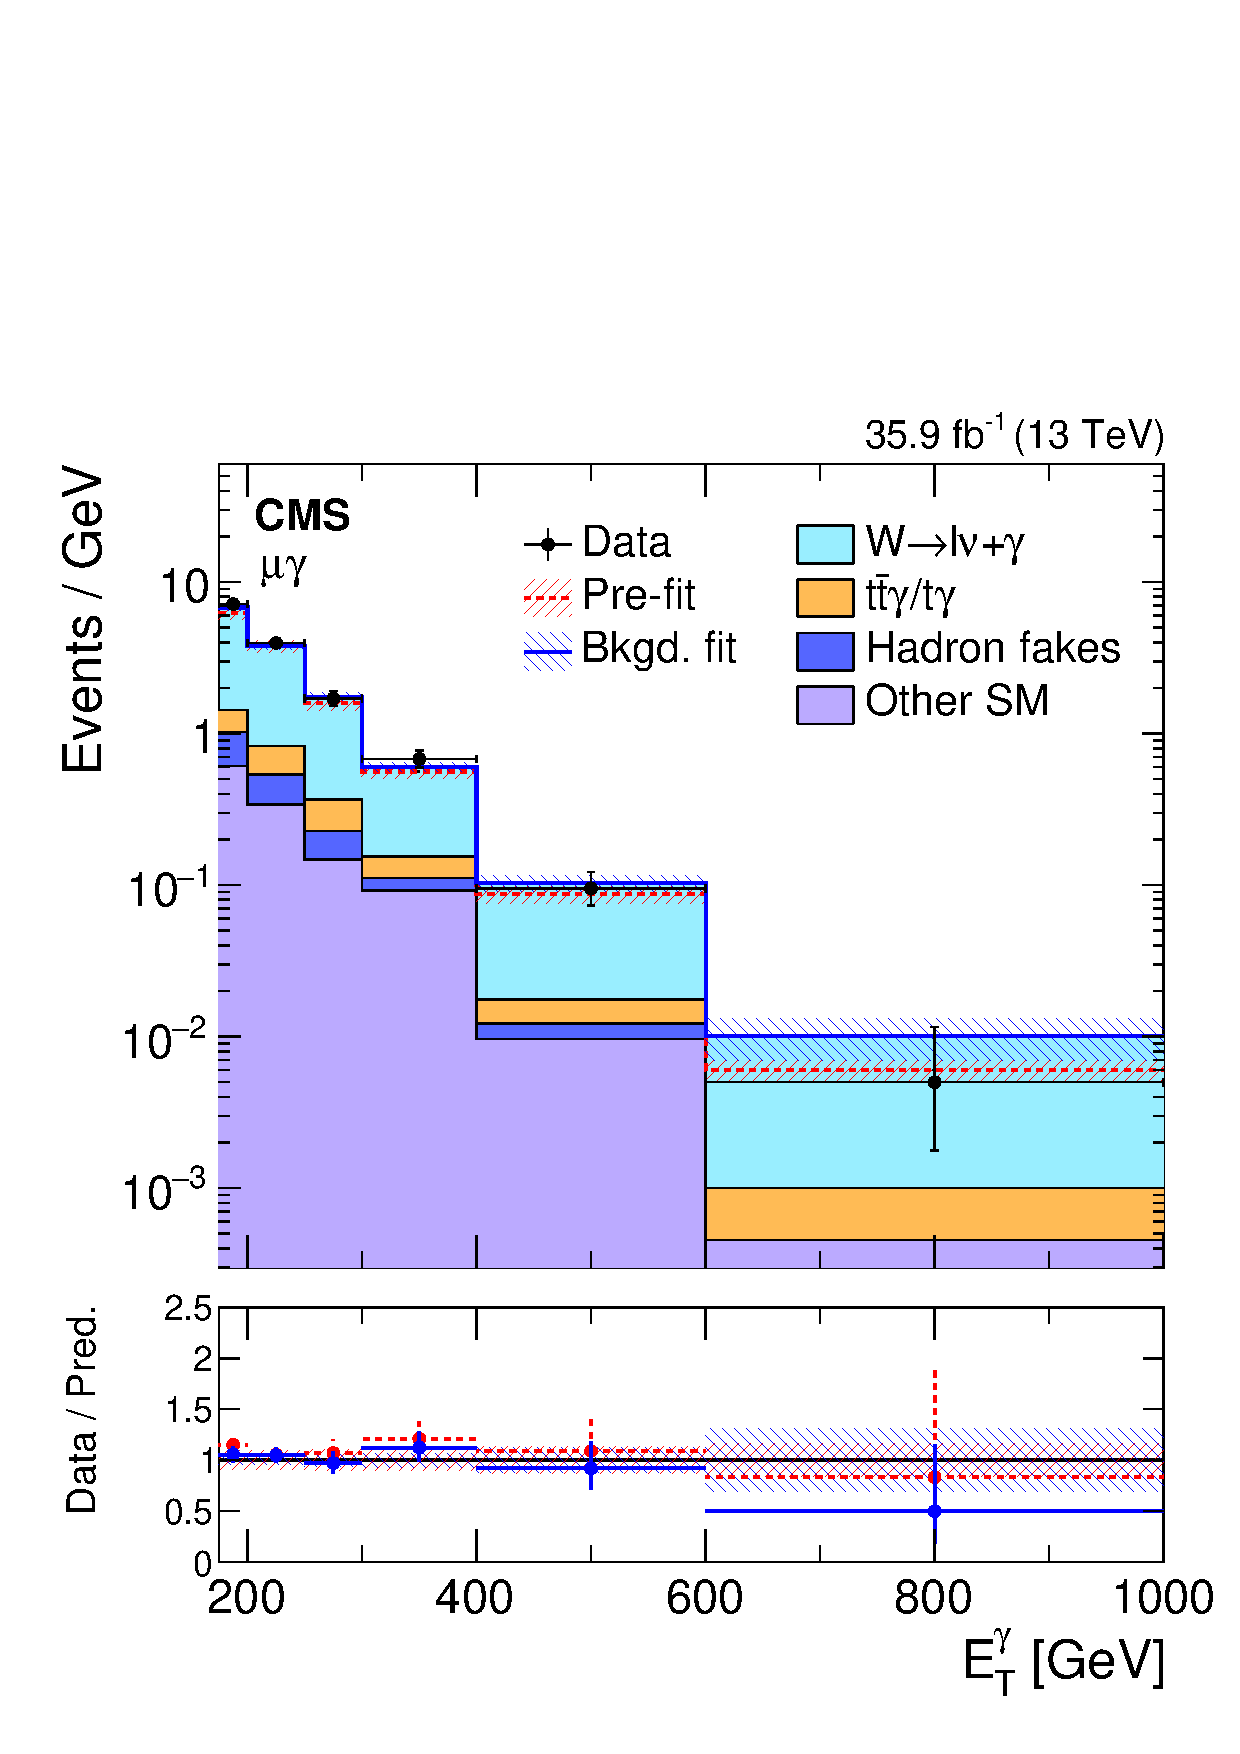
\includegraphics[width=0.45\textwidth]{Analysis/Figures/bonly_monomu.pdf}
    \caption{
      Comparison between data and MC simulation in the four control regions: 
      \Pe\Pe\Pgg\ (upper left), 
      \Pgm\Pgm\Pgg\ (upper right), 
      \Pe\Pgg\ (lower left), 
      \Pgm\Pgg\ (lower right) 
      before and after performing the simultaneous fit across all the control samples and signal region, and assuming absence of any signal.
      The last bin of the distribution includes all events with $\ETg > 1000\GeV$. 
      The ratios of data with the pre-fit background prediction (red dashed) and post-fit background prediction (blue solid) are shown in the lower panels. 
      The bands in the lower panels show the post-fit uncertainty after combining all the systematic uncertainties.
}
    \label{fig:postfitCR}
\end{figure}

\begin{figure}[htbp]
  \centering
    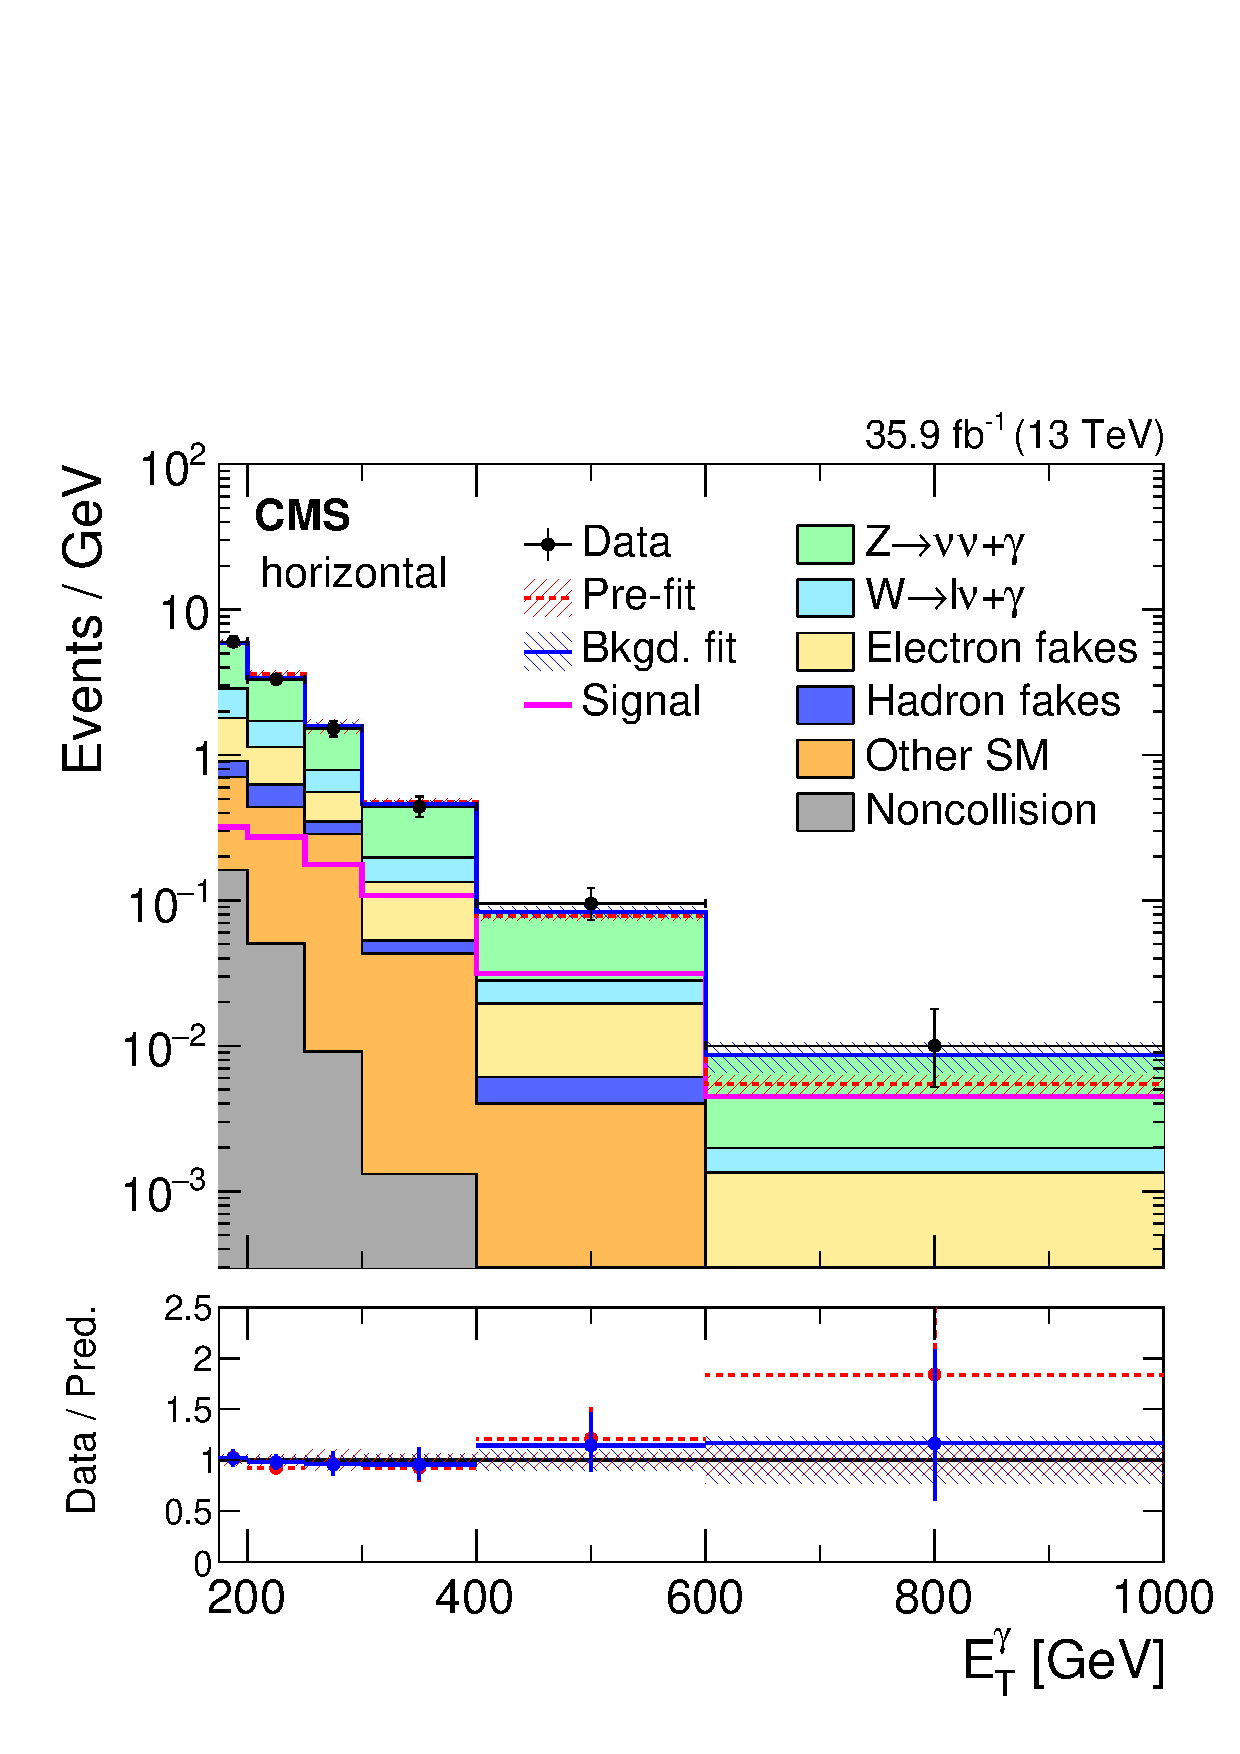
\includegraphics[width=0.45\textwidth]{Analysis/Figures/bonly_horizontal.pdf}
    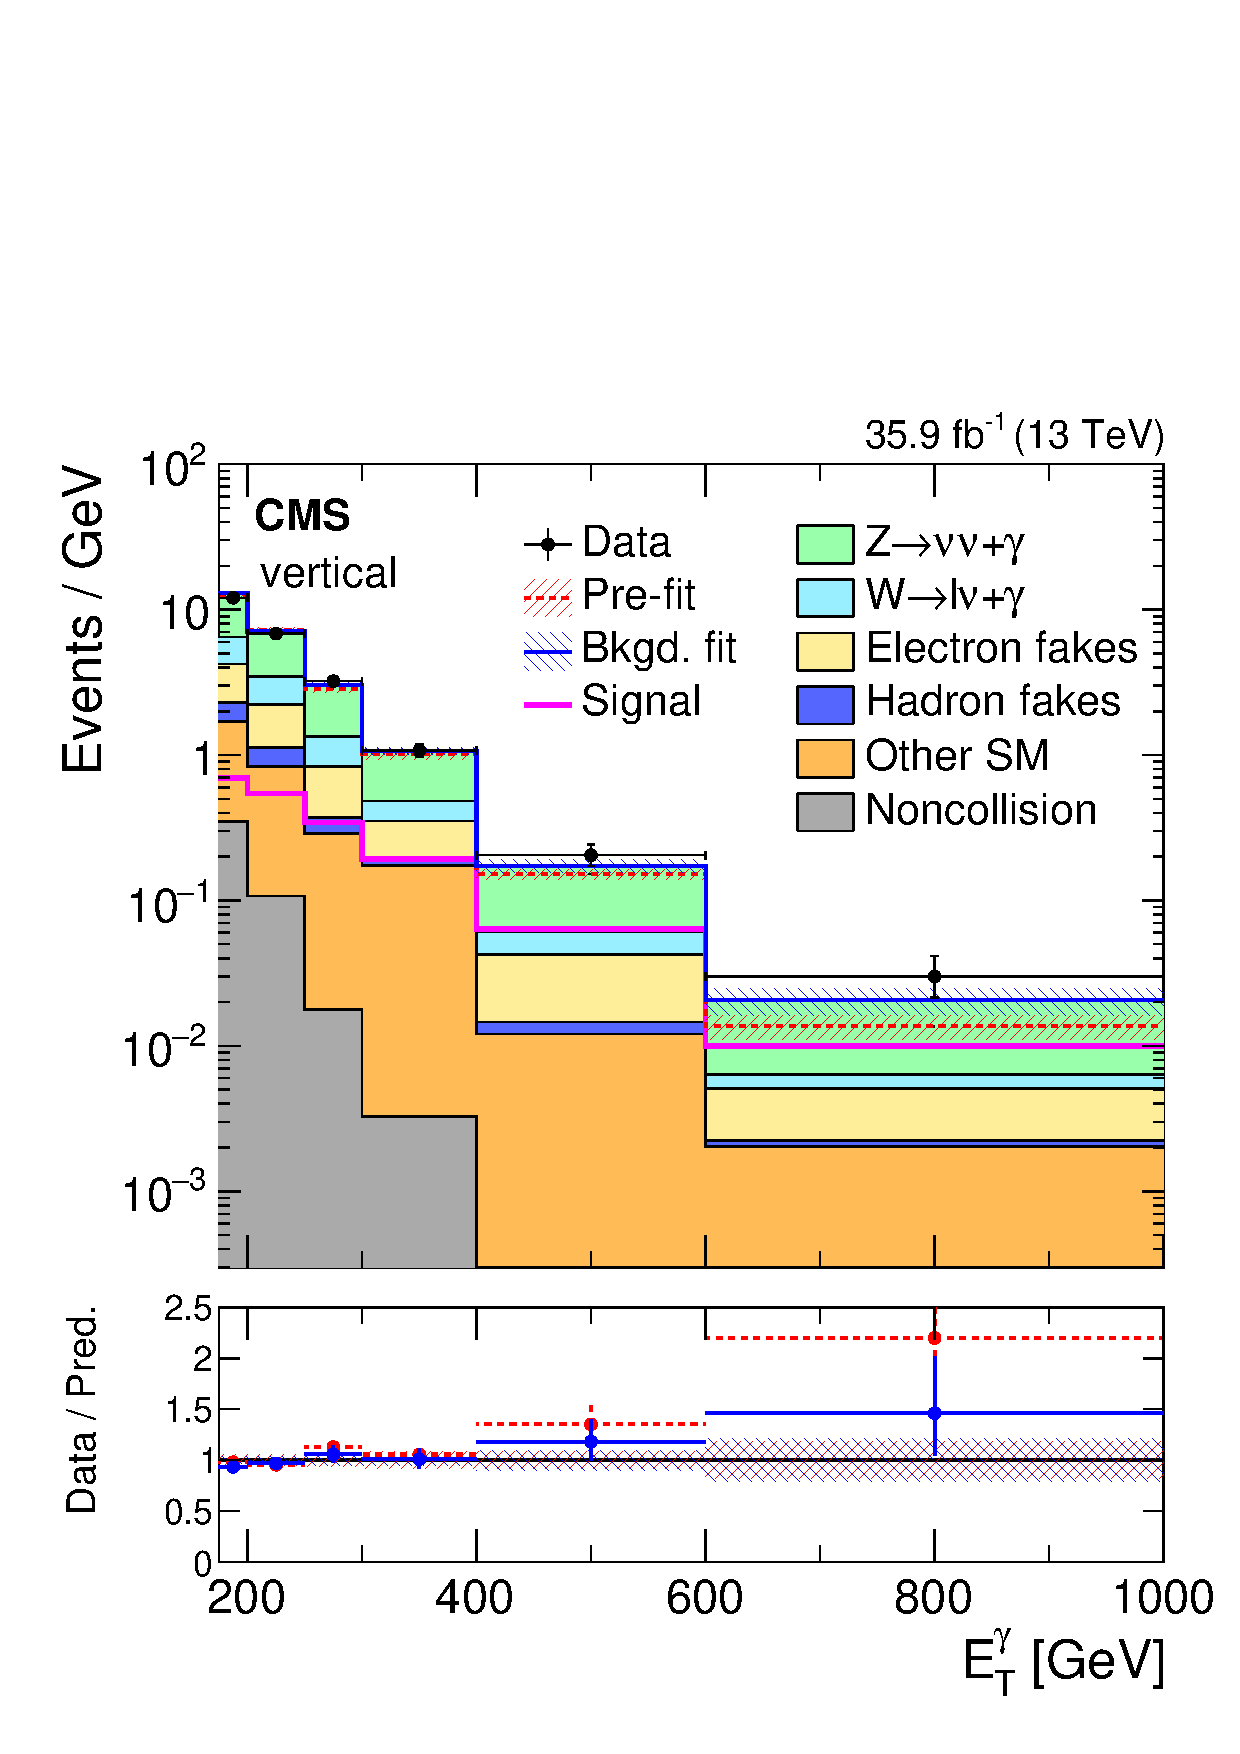
\includegraphics[width=0.45\textwidth]{Analysis/Figures/bonly_vertical.pdf}
    \caption{
      Observed \ETg\ distributions in the horizontal (left) and vertical (right) signal regions compared with the post-fit background expectations for various SM processes.
      The last bin of the distribution includes all events with $\ETg > 1000\GeV$. 
      The expected background distributions are evaluated after performing a combined fit to the data in all the control samples and the signal region. 
      The ratios of data with the pre-fit background prediction (red dashed) and post-fit background prediction (blue solid) are shown in the lower panels. 
      The bands in the lower panels show the post-fit uncertainty after combining all the systematic uncertainties. 
      The expected signal distribution from a 1\TeV vector mediator decaying to 1\GeV DM particles is overlaid.
    }
    \label{fig:postfitSR}
\end{figure}

Figure~\ref{fig:postfitCR} shows the observed \ETg\ distributionsin the four control regions compared with the results from simulations before and after performing the simultaneous fit across all the control samples and signal region, and assuming absence of any signal.
Figure~\ref{fig:postfitSR} shows the observed \ETg\ distributions in the horizontal and vertical signal regions compared with the results from simulations before and after performing a combined fit to the data in all the control samples and the signal region. 
The observed distributions are in agreement with the prediction from SM and noncollision backgrounds.

\begin{table}[htbp]
\centering
\caption{Expected event yields in each \ETg\ bin for various background processes in the horizontal signal region.
         The background yields and the corresponding uncertainties are obtained after performing a combined fit to data in all the control samples, excluding data in the signal region.
         The observed event yields in the horizontal signal region are also reported.}
\label{tab:yield_mask_horizontal}
\begin{tabular}{ lcccccc }
\hline
\rule[-1.2ex]{0pt}{3.8ex}\ETg~[\GeVns{}]      &         [175,  200] &         [200,  250] &         [250,  300] &         [300,  400] &         [400,  600] &         [600, 1000] \\
\hline
$\PZ\Pgg$        & $  81.2 \pm   8.0 $ & $  88.2 \pm   8.4 $ & $  38.8 \pm   4.8 $ & $  26.8 \pm   3.7 $ & $   8.8 \pm   1.9 $ & $   1.4 \pm   0.7 $ \\
$\PW\Pgg$        & $  27.9 \pm   3.7 $ & $  29.9 \pm   3.9 $ & $  11.4 \pm   1.7 $ & $   6.3 \pm   1.2 $ & $   1.4 \pm   0.4 $ & $   0.1 \pm   0.1 $ \\
Misid. electrons & $  22.5 \pm   2.7 $ & $  25.7 \pm   2.7 $ & $  10.5 \pm   1.0 $ & $   8.2 \pm   0.7 $ & $   2.7 \pm   0.2 $ & $   0.5 \pm   0.0 $ \\
Misid. hadrons   & $   5.2 \pm   2.2 $ & $   9.3 \pm   1.8 $ & $   3.1 \pm   0.7 $ & $   1.0 \pm   0.3 $ & $   0.4 \pm   0.1 $ & $   0.0 \pm   0.0 $ \\
Other SM         & $  13.6 \pm   2.0 $ & $  19.6 \pm   1.3 $ & $  13.9 \pm   0.4 $ & $   4.2 \pm   0.2 $ & $   0.8 \pm   0.0 $ & $   0.1 \pm   0.0 $ \\
ECAL spikes      & $   4.3 \pm   1.3 $ & $   2.7 \pm   0.8 $ & $   0.5 \pm   0.1 $ & $   0.1 \pm   0.0 $ & $   0.0 \pm   0.0 $ & $   0.0 \pm   0.0 $ \\
Total prediction & $ 154.6 \pm   8.3 $ & $ 175.4 \pm   8.8 $ & $  78.2 \pm   5.3 $ & $  46.6 \pm   4.0 $ & $  14.1 \pm   2.1 $ & $   2.1 \pm   0.8 $ \\
Observed         & $ 150   \pm  12   $ & $ 166   \pm    13 $ & $  76.0 \pm   8.7 $ & $  44.0 \pm   6.6 $ & $  19.0 \pm   4.4 $ & $   4.0 \pm   2.0 $ \\
\hline
\end{tabular}
\end{table}

\begin{table}[htbp]
\centering
\caption{Expected event yields in each \ETg\ bin for various background processes in the vertical signal region.
         The background yields and the corresponding uncertainties are obtained after performing a combined fit to data in all the control samples, excluding data in the signal regions.
         The observed event yields in the vertical signal region are also reported.}
\label{tab:yield_mask_vertical}
\begin{tabular}{ lcccccc }
\hline
\rule[-1.2ex]{0pt}{3.8ex}\ETg~[\GeVns{}]      &         [175,  200] &         [200,  250] &         [250,  300] &         [300,  400] &         [400,  600] &         [600, 1000] \\
\hline
$\PZ\Pgg$        & $ 172   \pm    17 $ & $ 190   \pm  18   $ & $  83   \pm  10   $ & $  58.6 \pm   7.9 $ & $  18.0 \pm   3.9 $ & $   3.1 \pm   1.6 $ \\
$\PW\Pgg$        & $  59.9 \pm   7.8 $ & $  63.6 \pm   7.8 $ & $  24.6 \pm   3.5 $ & $  13.4 \pm   2.4 $ & $   3.0 \pm   0.8 $ & $   0.3 \pm   0.2 $ \\
Misid. electrons & $  48.4 \pm   5.6 $ & $  56.2 \pm   5.1 $ & $  23.4 \pm   1.8 $ & $  15.7 \pm   1.4 $ & $   5.6 \pm   0.4 $ & $   1.2 \pm   0.1 $ \\
Misid. hadrons   & $  15.1 \pm   4.4 $ & $  14.5 \pm   3.1 $ & $   4.2 \pm   0.8 $ & $   2.3 \pm   0.8 $ & $   0.5 \pm   0.1 $ & $   0.1 \pm   0.1 $ \\
Other SM         & $  33.8 \pm   4.1 $ & $  36.6 \pm   2.7 $ & $  13.6 \pm   0.5 $ & $  17.1 \pm   0.6 $ & $   2.4 \pm   0.1 $ & $   0.8 \pm   0.0 $ \\
ECAL spikes      & $   9.3 \pm   2.8 $ & $   5.7 \pm   1.7 $ & $   0.9 \pm   0.3 $ & $   0.3 \pm   0.1 $ & $   0.0 \pm   0.0 $ & $   0.0 \pm   0.0 $ \\
Total prediction & $ 339   \pm  18  $ & $ 366   \pm  19   $ & $ 150   \pm  11   $ & $ 107.5 \pm   8.7 $ & $  29.6 \pm   4.3 $ & $   5.4 \pm   1.7 $ \\
Observed         & $ 301   \pm  17   $ & $ 342   \pm  19   $ & $ 161 \pm  13   $ & $ 107   \pm  10   $ & $  41.0 \pm   6.4 $ & $  12.0 \pm   3.5 $ \\
\hline
\end{tabular}
\end{table}

The expected yields in each bin of \ETg\ for all backgrounds in the horizontal and vertical signal regions after performing a combined fit to data in all the control samples, excluding data in the signal regions, are given in Tables~\ref{tab:yield_mask_horizontal} and~\ref{tab:yield_mask_vertical}, respectively.
The covariances between the predicted background yields across all the \ETg~bins in the two signal regions are shown in Fig.~\ref{fig:correlation_matrix}.
The expected yields together with the covariances can be used with the simplified likelihood
approach detailed in Ref.~\cite{CMS-NOTE-2017-001} to reinterpret the results for models not studied in this thesis

\begin{figure}[hbtp]
  \centering
  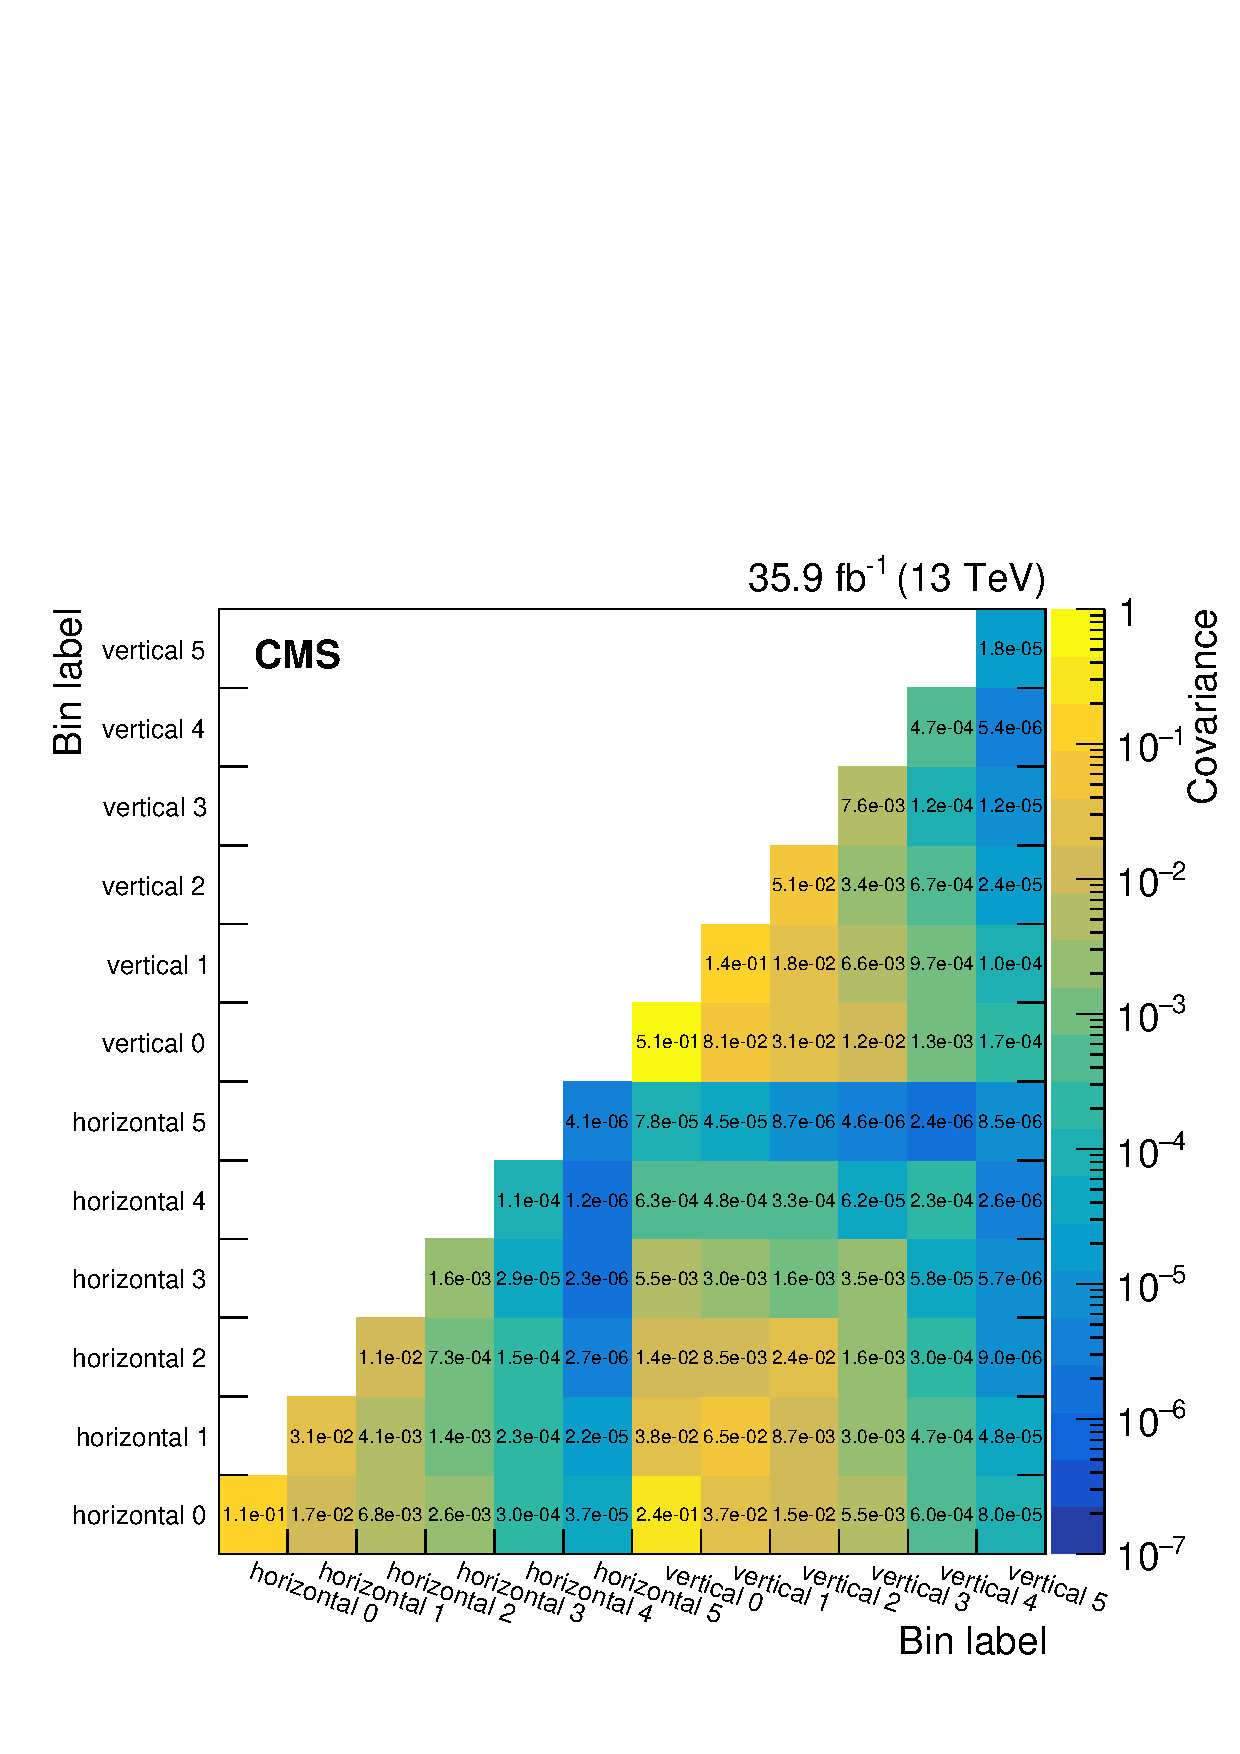
\includegraphics[width=0.9\textwidth]{Analysis/Figures/correlation_matrix.pdf}
  \caption{
    Covariances between the predicted background yields in all the \ETg\ bins of the horizontal and vertical signal regions.
    The bin labels specify which signal region the bin belongs to and what number bin it is for that region.}
  \label{fig:correlation_matrix}
\end{figure}.

\subsection{Limits}
\label{subsec:limits}

\begin{figure}[htbp]
  \centering
   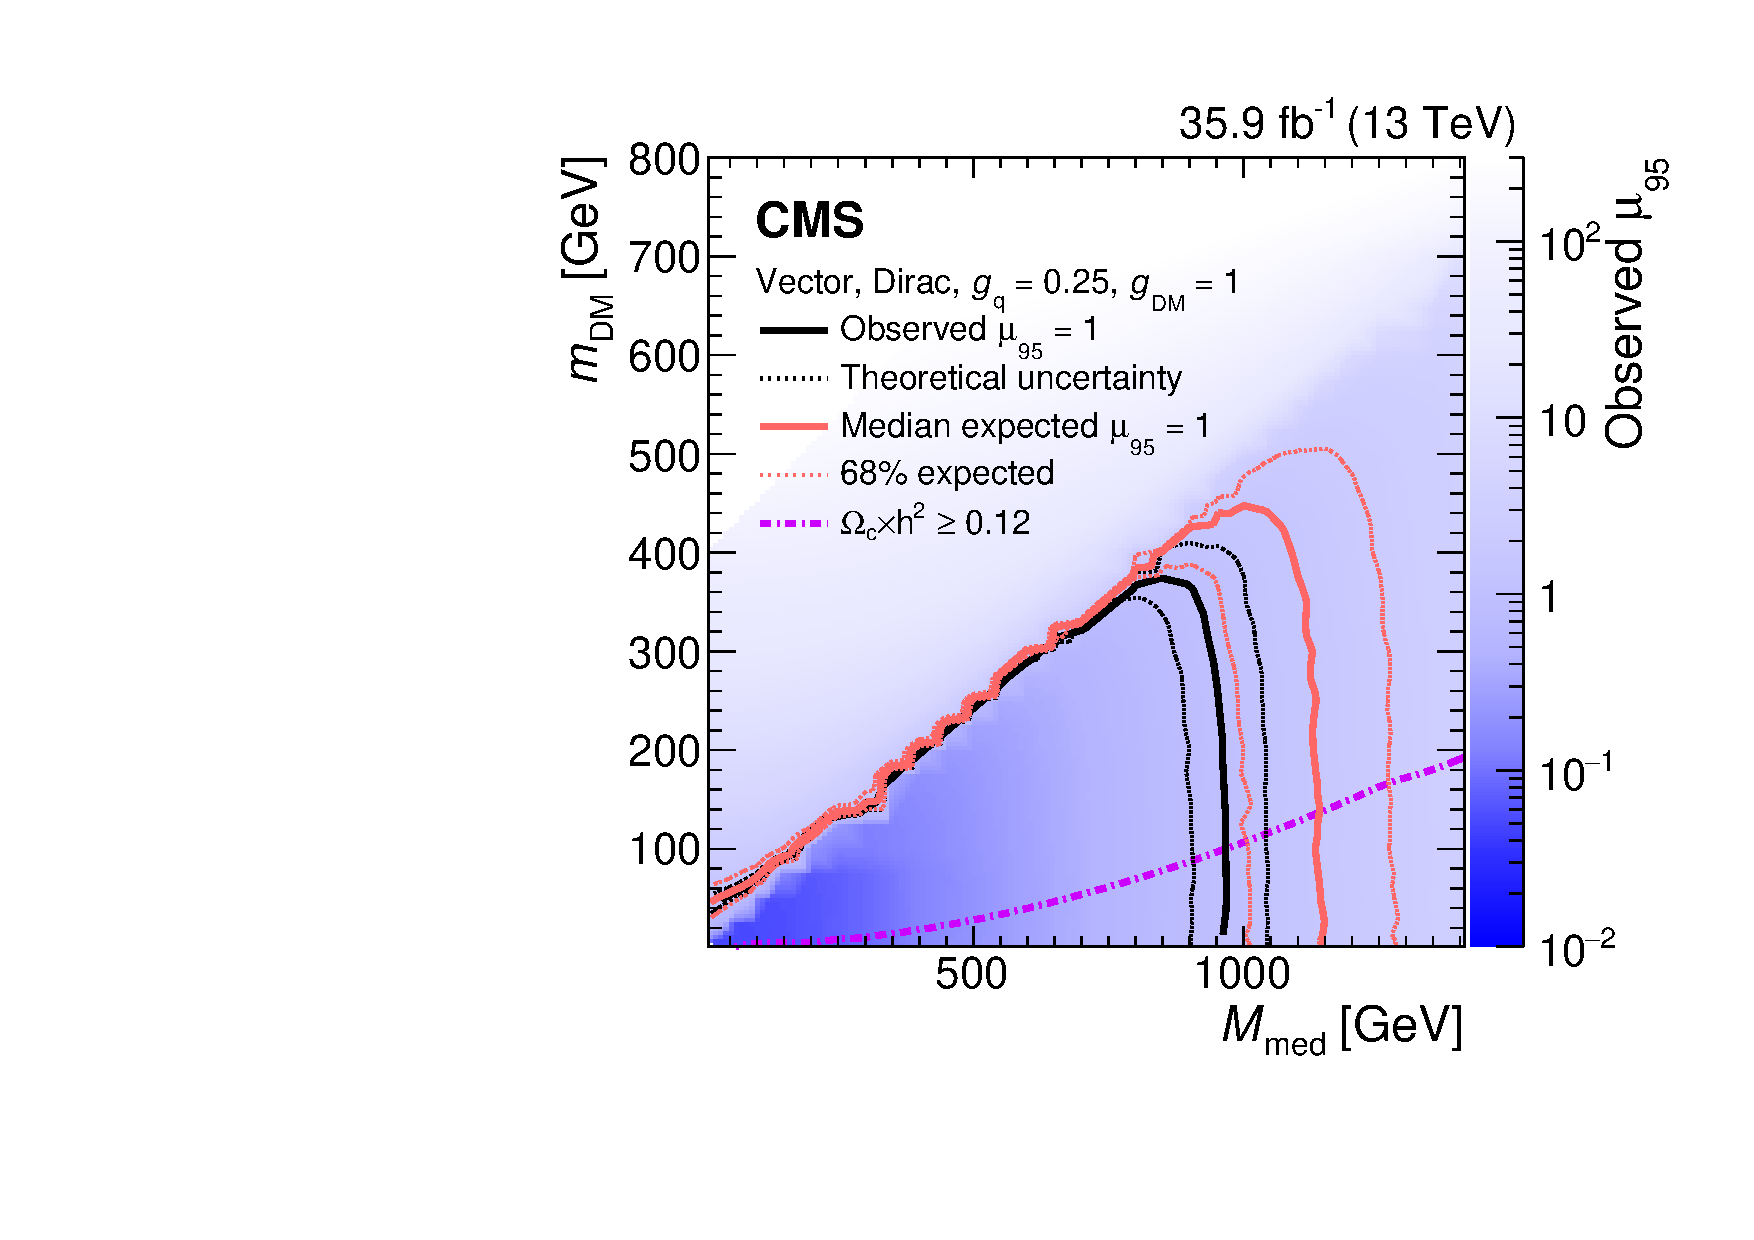
\includegraphics[width=0.48\linewidth]{Analysis/Figures/limits_vector.pdf}
    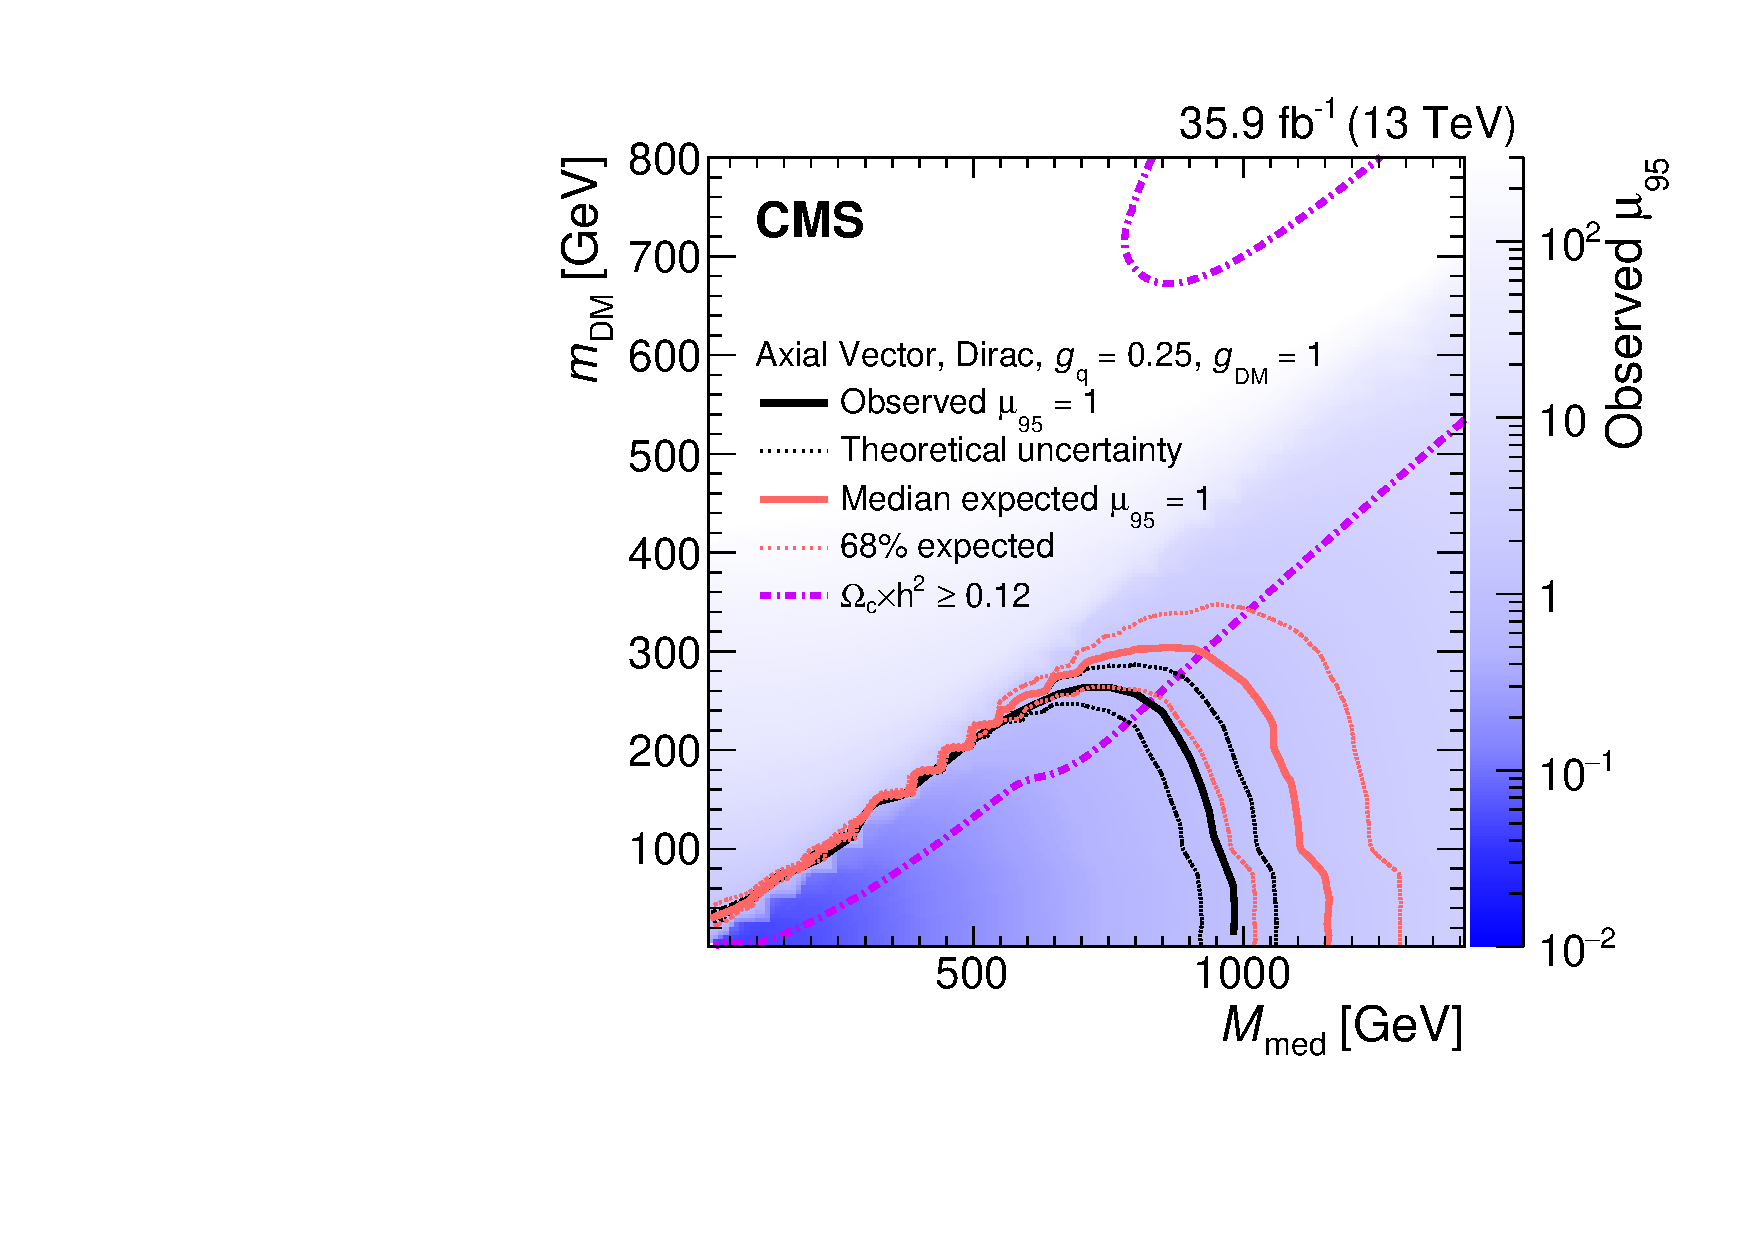
\includegraphics[width=0.48\linewidth]{Analysis/Figures/limits_axial.pdf}
    \caption{
      The ratio of 95\% \CL\ upper cross section limits to the theoretical cross section ($\mu_{95}$), for DM simplified models with vector (left) and axial-vector (right) mediators, assuming $\gq=0.25$ and $\gDM=1$.
      Expected $\mu_{95} = 1$ contours are overlaid in red. 
      The region under the observed contour is excluded. For DM simplified model parameters in the region below the lower violet dot--dash contour, and also above the corresponding upper contour in the right hand plot, cosmological DM abundance exceeds the density observed by the Planck satellite experiment.
    }
    \label{fig:limits}
\end{figure}

Figure~\ref{fig:limits} shows the 95\% \CL\ upper cross section limits with respect to the corresponding theoretical cross section ($\mu_{95}= \sigma_{95\%}/\sigma_{\text{theory}}$) for the  vector and axial-vector mediator scenarios, in the \mmed--\mdm\ plane. 
The solid black (dashed red) curves are the observed (expected) contours of $\mu_{95} = 1$. 
The $\sigma_{\text{theory}}$ hypothesis is excluded at 95\% \CL\ or above in the region with $\mu_{95} < 1$. 
The uncertainty in the expected upper limit includes the experimental uncertainties. 
For the simplified DM LO models considered, mediator masses up to 950\GeV are excluded for values of \mdm\ less than 1\GeV.
